\documentclass[thesis,tocnosub,noragright,centerchapter,12pt]{uiucecethesis09}

% Use draftthesis for notes and date markings on every page.  Useful when you
%   have multiple copies floating around.
% Use offcenter for the extra .5 inch on the left side. Needed with fullpage and fancy.
% Use mixcasechap for compatibility with hyperref package, which does NOT like all caps default
% Use edeposit for the adviser/committee on the title page.
% Use tocnosub to suppress subsection and lower entries in the TOC.
% PhD candidates use "proquest" for the proquest abstract.

\makeatletter

\usepackage[table,xcdraw]{xcolor}
\usepackage{setspace}
\usepackage{epsfig}  % for figures
%\usepackage{graphicx}  % another package that works for figures
%\usepackage{subfigure}  % for subfigures
\usepackage{amsmath}  % for math spacing
%\usepackage{amssymb}  % for math spacing
%\usepackage{url}  % Hyphenation of URLs.
\usepackage{lscape}  % Useful for wide tables or figures.
\usepackage{apacite}
\usepackage{natbib}
\usepackage[justification=raggedright]{caption}	% makes captions ragged right - thanks to BryceLobdell

\usepackage{graphicx}
\graphicspath{ {Images/} }

% Uncomment the appropriate one of the following four lines:
\msthesis
phdthesis
%\otherdoctorate[abbrev]{Title of Degree}
%\othermasters[abbrev]{Title of Degree}

\title{The Devolution of Cooperation: A Framework for Analyzing the Sustainbility of Collective Action in Science Commons}
\author{Nicholas M.Weber}
\department{Graduate }
\degreeyear{2014}

% Advisor name is required for
% - doctoral students for the ProQuest abstract
% - master's students who do not have a master's committee
\advisor{Your Adviser Here}

% Uncomment the \committee command for
% - all doctoral students
% - master's students who have a master's committee
%\committee{Professor Firstname Lastname, Chair\\
%        Professor Firstname Lastname} % etc.

\begin{document}

%%%%%%%%%%%%%%%%%%%%%%%%%%%%%%%%%%%%%%%%%%%%%%%%%%%%%%%%%%%%%%%%%%%%%%%%%%%%%%%
% COPYRIGHT
%
%\copyrightpage
%\blankpage

%%%%%%%%%%%%%%%%%%%%%%%%%%%%%%%%%%%%%%%%%%%%%%%%%%%%%%%%%%%%%%%%%%%%%%%%%%%%%%%
% TITLE
%
\maketitle

%\raggedright
\parindent 1em%

\frontmatter

%%%%%%%%%%%%%%%%%%%%%%%%%%%%%%%%%%%%%%%%%%%%%%%%%%%%%%%%%%%%%%%%%%%%%%%%%%%%%%%
% ABSTRACT
%
\begin{abstract}
% Put the abstract in a file called "abs.tex" and it'll be inputted here.
\section{Abstract}

The sustainability of eScience research infrastructures is an increasingly complex problem addressed by science and technology policy. Through a case study of the International Comprehensive Ocean and Atmosphere Dataset (ICOADS) I describe a common property regime for sharing and pooling resources across traditional organizational boundaries, and the collective action needed to sustain this cooperative arrangement in the face of political, social, and economic change. I use this work to support the testing and refinement of an analytical framework. The contribution of this work will be a better understanding of how institutions for collective action evolve, and a framework for reducing the complexity of studying eScience commons.

\end{abstract}


%%%%%%%%%%%%%%%%%%%%%%%%%%%%%%%%%%%%%%%%%%%%%%%%%%%%%%%%%%%%%%%%%%%%%%%%%%%%%%%
% DEDICATION
%
\begin{dedication}
% Whatever dedication you want.

\begin{figure}
\centering

\includegraphics{cc0}
\end{figure}
\end{dedication}

%%%%%%%%%%%%%%%%%%%%%%%%%%%%%%%%%%%%%%%%%%%%%%%%%%%%%%%%%%%%%%%%%%%%%%%%%%%%%%%
% ACKNOWLEDGMENTS
%
% Put acknowledgments in a file called "ack.tex" and it'll be inputted here.
\begin{acknowledgments}
\input{ack}
\end{acknowledgments}

%%%%%%%%%%%%%%%%%%%%%%%%%%%%%%%%%%%%%%%%%%%%%%%%%%%%%%%%%%%%%%%%%%%%%%%%%%%%%%%
% TABLE OF CONTENTS
%
\tableofcontents

%%%%%%%%%%%%%%%%%%%%%%%%%%%%%%%%%%%%%%%%%%%%%%%%%%%%%%%%%%%%%%%%%%%%%%%%%%%%%%%
% LIST OF TABLES
%
% The List of Tables is not strictly necessary. Omitting the List of Tables will
% simplify the thesis check and reduce the number of corrections.
\listoftables

%%%%%%%%%%%%%%%%%%%%%%%%%%%%%%%%%%%%%%%%%%%%%%%%%%%%%%%%%%%%%%%%%%%%%%%%%%%%%%%
% LIST OF FIGURES
%
% The List of Figures is not strictly necessary. Omitting the List of Figures will
% simplify the thesis check and reduce the number of corrections.
\listoffigures

%%%%%%%%%%%%%%%%%%%%%%%%%%%%%%%%%%%%%%%%%%%%%%%%%%%%%%%%%%%%%%%%%%%%%%%%%%%%%%%
% LIST OF ABBREVIATIONS
%
% The List of Abbreviations is not strictly necessary.
\chapter{LIST OF ABBREVIATIONS}

%\begin{symbollist*}
%\item[EPIC] Explicitly Parallel Instruction Computing
%\item[GPU] Graphics Processing Unit
%\item[VLIW] Very Long Instruction Word
%\end{symbollist*}


%%%%%%%%%%%%%%%%%%%%%%%%%%%%%%%%%%%%%%%%%%%%%%%%%%%%%%%%%%%%%%%%%%%%%%%%%%%%%%%
% LIST OF SYMBOLS
%
%\begin{symbollist}[0.7in]
%\item[$\tau$] Time taken to drink one cup of coffee.
%\end{symbollist}

\mainmatter

%%%%%%%%%%%%%%%%%%%%%%%%%%%%%%%%%%%%%%%%%%%%%%%%%%%%%%%%%%%%%%%%%%%%%%%%%%%%%%%
% INSERT REAL CONTENT HERE
%

\chapter{}
}
In fields that study complex physical systems,
such as climate science, the production of reliable knowledge is often
beyond the capabilities of any one person or group. To overcome these
individual limitations climate science engages
in a form of collective action where many people, institutions, and
organizations effectively cooperate to share information and pool
resources in pursuit of a common goal \citep{oliver1993critical}. Increasingly this work is made
possible by access to publicly funded infrastructures, including
archives of openly accessible data, suites of open-source software, and
high performance computing facilities \citep{berman2013will}. Many of
these infrastructures are funded by government subsidies in the form of
research grants or cooperative agreements between a federal agency and a
research laboratory \citep{sarewitz2010frontiers}. A substantive
question for science and technology policy makers is how to best support these emerging arrangements so that investments in infrastructure and other durable resources are beneficial to the immediate needs of basic science research, but are also sustainably
managed and preserved for the benefit of future generations.\\

Although there is an abundance of literature that addresses collective action in scientific collaborations 
 \citep[e.g.][]{sonnenwald2007scientific} this work tends to focus on variables
leading to the success or failure of these arrangements \citep[e.g.][]{finholt2002collaboratories}, and therefore draws conclusions about how to design \emph{new}
infrastructures to support eScience research \citep{jirotka2013supporting}.
Few studies have looked at the sustainability of these cooperative arrangements, how
they evolve over time, or how the design of policies that underlie the
effective functioning of these collaborations in turn impact the ability
of diversely motivated groups to solve collective action problems.\\

\section{Research Questions}

This dissertation will develop a case study of the International
Comprehensive Ocean and Atmosphere Dataset (ICOADS), a cooperative project that develops, distributes and has sustained
an archive of marine climate information (data, software, documentation,
etc) over a thirty year period. This case study will provide a valuable understanding of the
ways in which scientific institutions for collective action evolve in
the face of social, political, and economic change.\\

The specific research questions that this case study addresses are:

\begin{quote}
\textbf{RQ1} : How does ICOADS, as an institution for collective action,
overcome transaction costs in organizing its production of new
knowledge?
\end{quote}

\begin{quote}
\textbf{RQ2} : How has ICOADS, as a project with particular
governance arrangements, evolved in response to external pressures from
funding agencies, the politicization of climate related research, and
rapid technological change?
\end{quote}

A major argument of this proposal is that science and technology policy
struggles to reliably address issues of sustainability, in part, because
social scientists studying cyberinfrastructure development, data sharing
and reuse, or eScience collaboration more generally, have failed to
provide an adequate base of knowledge for decision makers to consult
in designing policy interventions
\citep{miller2013facto}. This is not because this work lacks in quality
or relevant research findings, but as a result of these studies being so different in the levels and units of analysis, the presentation of findings, and disciplinary cultures that privilege theory construction over policy relevance.Too often valuable knowledge about governance, and the role of federal policy in successfully functioning collaborative arrangement remains isolated and difficult to meaningfully integrate \citep{jackson2013cscw, jackson2014policy}.\\

If science and technology policy is to move beyond simple
panaceas for solving the complex interrelated problems of sustaining
sociotechnical systems then it requires integrating knowledge from many different studies of cooperation, coordination and collaboration in eScience. I argue that this can be accomplished in developing analytical frameworks that specify a set of variables to be studied, and the different levels of interactions that are to be analyzed across cases. This requires frameworks that are flexible enough to be used in a variety of settings and by a
diverse number of researchers, and yet rigid enough to produce findings
that are comparable to one another in meaningful ways. The challenge for this approach is, as Jirotka, Lee and Olson recently put it, ``finding ways to make the complexity of socio-technical e-Science configurations more tractable without being reductionist'' \citeyearpar[p. 31]{jirotka2013supporting}.\\

Institutional scholars working in diverse fields like land and fisheries management,
ecology, and political science have for many years been successful at
producing frameworks for the analysis of sustainability in socio-economic settings \citep{ostrom2007institutional}. This is accomplished by leveraging systems and complexity theory
\citep{ostrom2007diagnostic} to identify concepts like stock flows, feedback loops, and
emergent properties that reductionist thinking often simplifies or
overlooks \citep{meadows2008thinking}. My third research question then asks:

\begin{quote}
\textbf{RQ3}: How can analytical frameworks successful for studying
collective action problems in other domains be modified for
sociotechnical settings where issues of sustainability, cooperation and
shared resource management are diverse and shifting over time?
\end{quote}

In the rest of this chapter, I argue that these are particularly relevant
questions to ask about institutions that are facing budget crises as a
result of the politicization of climate research, and that the
International Comprehensive Ocean and Atmosphere Data Set (ICOADS) project is an appropriate subject for this work. 

\section{ICOADS}

The International Comprehensive Ocean and Atmosphere Dataset (ICOADS) is
a cooperative project that curates, develops and distributes quality controlled
data, metadata, historical documentation, and software to the
climatology community. The project, originally named COADS, was
initiated in 1981 by researchers at the Earth System Research Laboratory
(ESRL), the National Climatic Data Center (NCDC), and the National
Center for Atmospheric Research (NCAR). Over time the project grew to
include international collaborators, and the name was changed to
International COADS in order to reflect the contributions of organizations like
the Joint World Meteorological Organisation (WMO), the Intergovernmental
Oceanographic Commission (IOC), and the Technical Commission for
Oceanography and Marine Meteorology (JCOMM).\\

Contemporary data curated by ICOADS come from a variety of sources,
including the Global Telecommunications System (GTS), in-situ
measurements taken by sea-faring vessels, earth observing satellites,
and both drifting and moored buoys. Historical data come from the
original 1981 effort to aggregate existing marine data records from
maritime archives around the world, as well as a continual stream of
historical records that have been rediscovered, or newly digitized. Data sources also now include the use of crowdsourcing efforts to transcribe weather recordings taken by military, shipping,
and whaling voyages from the 17th, 18th, and 19th century\footnote{To give some indication of how much the project has grown over time, the
first release of COADS data products contained 73 million records with
dates reaching back to 1852. As more shipping records have been
discovered and digitized the coverage of ICOADS has been extended to
1662, and now includes more than 261 million records. \citep{woodruff2011icoads}} \citep{brohan2009marine}.\\

The labor-intensive process of taking heterogeneous records from
different observing platforms, and uniformly processing and integrating the
data into a larger set of historical observations is the major value of
ICOADS ongoing work. This includes the preservation of provenance
metadata that is recorded for each individual record, allowing for
researchers to trace backwards in time to verify whether the source of a
supposed climate anomaly is genuine or the result of a data processing
error.\\

\subsection*{ICOADS Funding}

The production of ICOADS was originally meant to fill a gap in climate
change research which lacked an authoritative source of data for the
boundary conditions occurring at the ocean and atmosphere interface.
Although this was widely acknowledged as an important next step in earth
systems research, ICOADS partners struggled to attract funding for their
work. As a preface to the first release of COADS one of
the principle investigators noted that, ``It has taken four years and
much effort by many individuals and several institutions to obtain and
process the hundreds of tapes containing the basic data input. All of
this effort was provided from ongoing activities; there was no
appropriation identified for the task. It is a tribute to the spirit of
cooperation among the participating organizations that the task has been
successfully completed'' \citep{slutz1985comprehensive}. Even though the project
was unfunded the developers of ICOADS release 1.0 committed to making
all of its products (data, software, etc.) freely available to the
climate science community \citep{worley2005icoads}.\\

Free and open access to ICOADS has helped it become recognized by the
climate community as ``the most complete and heterogeneous collection of
surface marine data in existence'' \citep{woodruff2011icoads}. ICOADS data
have been used extensively in earth systems science research,
international climate assessments such as the IPCC AR4 and AR5 reports,
as well as reanalysis projects that
combine historical weather observations with climate data to create
authoritative datasets for the climate modeling community \citep{kalnay1996ncep}. However, the success and widespread use of ICOADS has not resulted in
greater stability for the funding of the project. This is due in part to
the difficulty in calculating the research impact of many different ICAODS products
\citep{weber2014coop}, as well as an overall
decrease in federal funding for the maintenance of
research infrastructures \citep{berman2013will}. The politicization of climate related research has also impacted
ICOADS funding in recent years. In the winter of 2012, this became a major issue for the
sustainability of the project, as NOAA announced that:

\begin{quote}
For budgetary reasons, stemming from pending large cuts at the NOAA
Climate Program Office (CPO), ESRL Directors have determined that it is
no longer feasible for its Physical Science Division (PSD) to continue
supporting any further ICOADS work-- effective immediately \citep{icoads2012}.
\end{quote}

By operating as a cooperative, funding would still be available for the
maintenance and curation of ICOADS data through NCAR (NSF), but the
project could not plan major updates to the software or documentation
that complements ICOADS data, and a much anticipated third release was
delayed indefinitely.\\

\subsubsection*{Studying the ICOADS Community}

My work with the ICOADS community began as an Advanced Studies Program
(ASP) fellow at NCAR in the summer of 2012. I was originally interested
in asking research questions about the evaluation of federally funded
research and development centers (FFRDCs), and the co-production of
knowledge between climate scientists and policy
makers. My initial work on these questions took a grounded theory
approach \citep{corbin2008basics}, using NOAA's defunding of ESRL as a critical incident to
ask questions about how ICOADS was evaluated by policy makers, and its
general impact or importance to knowledge production in climate science
\citep{flanagan1954critical}.\\

Below, I present findings from this work. I
describe how these studies helped me to generate a new set of research
questions about public goods, collective action, and the sustainability
of cooperative work more generally. Each of the studies described below
were collaborations with software engineers and project scientists at
NCAR, as well as colleagues at the Center for Informatics Research in
Science and Scholarship (CIRSS). However, I conceived of and designed
each study, conducted the majority of all data analysis, and I am the
first author on all but one of the resulting publications from this work
(of which I am the co-first author).

\section{The Data Usage Index}

Federally funded research and development centers typically measure the
levels of service they provide to end users through descriptive
statistics, such as the number of times a data file has been downloaded
over a given period of time. To better understand the use of ICOADS in
the climate science community my first research project used log
analysis techniques from Information Science \citep{jansen2006search, nicholas2005scholarly}, and in particular a Data Usage Index (hereafter referred to as DUI) used in the
life sciences. The DUI was originally designed to measure the impact of
institutional contributions to the Global Biodiversity Information Federation
Database (GBIF) by using \emph{indicators} of how data were discovered and accessed (i.e.~number of
downloads, page hits, files contributed by an institution, etc.) \citep{chavan2009towards}. In the DUI, indicators are extracted from user query logs and combined in simple, but unique ways to calculate impact
factors \citep[; See Appendix A, Table 1]{ingwersen2011indicators}.\\

Initially, our work aimed to modify the DUI's indicators from the
context of a biodiversity database to the Research Data Archive (RDA) at
NCAR, which hosts and serves climate data and software (including
ICOADS). To do this we developed a set of use cases based on a
researcher's discovery, selection, and mode of access to different data
products from the RDA.\\

From the use cases we identified six key indicators that were captured
in the RDA's logs, as well as potentially informative relationships
between these indicators (see Table 1 below).\\
\\
\begin{table}[h]
\resizebox{\textwidth}{!}{%
\begin{tabular}{llll}
\textbf{Code}   & \textbf{Indicator}        & \textbf{Explanation}                                         &  \\
uu(ds)          & Unique Users              & Unique users that downloaded data during a time window       &  \\
n(ds)           & Number of Datasets        & Number of Datasets assigned DS number by RDA                 &  \\
f(ds)           & Files DS                  & Number of files in Dataset per time window                   &  \\
d(ds)           & Download Frequency        & Total number of files downloaded per time window             &  \\
hp(ds)          & Homepage Hits             & Home Page Hits of Data Set per time window                   &  \\
d(ds) /uu (ds)  & Download Density          & Average number of files downloaded per unique user           &  \\
d(ds) / f (ds)  & Usage Impact              & Total number of downloaded files over total files in dataset &  \\
d(ds) / hp(ds)  & Usage Balance             & Files downloaded by number of homepage hits per time window  &  \\
hp(ds) / f(ds)  & Interest impact           & Total homepage hits per number of files in dataset           &  \\
hp(ds) / uu(ds) & Secondary Interest Impact & Total Homepage hits over unique users                        &  \\
ss(ds) / d(ds)  & Subset Ratio              & Subset requests over total number files downloaded           & 
\end{tabular}
}
\end{table}\\

The completed use cases also demonstrated that two user types could be
identified based on how data were accessed:

\begin{itemize}
\item
  \textbf{Programmatic Users}: accessed or downloaded data through a
  command line tool (e.g. `-curl {[}\^{}curl{]} or 'wget'
  {[}\^{}wget{]}) or through a scripting language.
\item
  \textbf{Assisted Users:} access data via the graphical user interface,
  or by subset requests made through a separate tool developed by the
  RDA staff.
\end{itemize}

\textbf{Methods}\\
To test the effectiveness of the modified DUI three
different RDA data products were selected - including the most recent
release of ICOADS (version 2.5). Indicators from the completed use-cases
were then extracted from the user logs of each dataset over a sixteen
month period. This resulted in an index for each of the three datasets
(See Appendix A).\\

From the index of each dataset we then further calculated two impact
factors:\\

  \textbf{Usage Impact Factor}
  \begin{equation}
  (d(u) / f(u))/\sum_{1}^{n}{d}/\sum_{1}^{n}{f}
  \end{equation}
  where (u) is the given resource unit, (d)
  is the download frequency of users, (f) is the number of files
  downloaded per user session, and (n) is the total number of units (files
  available in the dataset) in the denominator.\\
  
  \textbf{Interest Impact Factor}\begin{equation}
  (hp(u) / f(u))/\sum_{1}^{n}{hp}/\sum_{1}^{n}{f}
  \end{equation} which is identical to UIF except
  download frequency (d) of users is replaced by the number of homepage
  hits (hp) a dataset receives.\\

\textbf{Outcomes}\\

The Usage and Interest Impact Factor scores that we calculated were not significant for any of our use caes.  This ultimately led us to conclude
that these metrics were not valid for policy related impact assessments.
However, the indexes did prove to be a useful tool in tracking
curatorial interventions \citep{weber2013product}. RDA curators were able to
use the indexes to better understand usage patterns within different
data communities, and to explore changes in the way that a dataset was
accessed over time. As an example of the latter point, the ICOADS Usage
Impact Factor scores declined over the sixteen month period of our study; dropping
significantly before the summer of 2011 and continuing at a low rate
through 2012. A long-time curator of ICOADS explained that this could be
the result of having added new software to the repository that spring.
This software was developed to help users subset new ICOADS data that
were formatted differently from previous releases. The software was
meant to decrease the total number of files a user needed to download,
and speed up applications built to regularly harvest data from the RDA.\\

We investigated this hypothesis by dividing the indicator scores based
on the two user types (programmatic and assisted). After doing this, we
observed a significant upward shift in the total number of programmatic
users of ICOADS, and an overall decrease in the number of
files that were downloaded over the same time period. We also found a number of
modifications of the software posted to on-line discussion forums for
ICOADS\footnote{To be cautious, what we observed in this instance
is a loose correlation between user types and the total amount of files
downloaded. We don't know with any amount of statistical certainty that
the introduction of new software caused users to become more efficient
in their downloading, and without further examples of this phenomena we
can't say whether or not the finding would be replicated in other
communities}.\\

That the software increased the efficiency of the archive, but
simultaneously decreased the impact factor scores seemed logical - this
was a result of the designer of the study (me) not understanding the
function of the archive well enough to develop a robust set of impact
metrics. But, finding modifications of the software posted to public
repositories was puzzling. If the research environment is so
competitive that ICOADS was being defunded then why would researchers, all of whom are interested in the same resource, help each other to work more efficiently? \\

To put this into economic terms, obtaining information assets in the
ICOADS community requires users to exchange and share a number of
\emph{transaction costs}. In organizing economic productivity, individual actors
are typically able to overcome high transaction costs in one of two ways: through a
marketplace where prices are ``naturally borne out'' of exchange and so
individuals follow pricing signals, or by coordinating their actions
through a firm where individuals follow a hierarchy of decision making \citep{coase1937nature, williamson1975markets}.\\

In looking at the small example of software modification it appears that
neither model explains how the ICOADS community organizes itself to
overcome transaction costs. These unselfish acts also directly contradict the private property, self-interested model being used to
describe resource sharing in other eScience settings \citep[e.g.][]{birnholtz2003data, zimmerman2008new, wallis2013if}.
For ICOADS, overcoming transaction costs in producing new knowledge seemed more
similar to open-source software projects, and what Benkler called
\emph{commons-based peer production}, where economic productivity is
``radically decentralized, collaborative, and nonproprietary; based on
sharing resources and outputs among widely distributed, loosely
connected individuals who cooperate with each other without relying on
either market signals or managerial commands'' \citeyearpar[p. 60]{benkler2006wealth}.\\

In working with colleagues at NCAR my observations about the unique way
in which ICOADS is produced led to the first research question to be
answered in this dissertation:\\

\textbf{RQ1} : How does ICOADS, as an institution for collective action,
overcome transaction costs in organizing its production of new
knowledge? If peer production is indeed the model by which this is
achieved:

\begin{itemize}
\itemsep1pt\parskip0pt\parsep0pt
\item[]
  RQ 1.1 How, and/or in what ways does it differ form other forms of
  peer production?
\item[]
  RQ 1.2 How does ICOADS sustain these successful cooperative
  arrangements?
\item[]
  RQ 1.3 What are the activities of its community members necessary to
  achieve this sustained success, and how can those actions be
  recognized, either formally or informally, over the duration of the
  project's existence?
\end{itemize}

\section{The Genealogy of ICOADS}

ICOADS is widely reused in developing new climatology data products, but
tracking the reuse of ICOADS through citation analysis is limited
by the inconsistency in how the project is acknowledged,  and what is subsequently cited (e.g.The dataset hosted at the RDA?, A
paper describing the dataset?, By thanking individual curators in an acknowledgment section?) (Weber, Mayernik, and Worley, 2014).\\

To better understand the history of how ICOADS has been reused, we conducted a second study using techniques from the field
of evolutionary biology \citep{page2009molecular} and cultural analytics \citep{mace2005phylogenetic} to produce a
genealogy of ICOADS. Our inspiration for this work came from a set of
studies that looked at the history of climate models by tracing their
relatedness (See Figure 1.1); The figure on the left is from a study
conducted by Edwards, who created a ``family tree'' of Atmospheric
General Circulation Models (AGCM) from archival documents and oral
histories \citeyearpar{edwards2010vast}. The figure on right is a dendrogram
showing relatedness of climate models that participated in the 5th
Climate Model Intercomparrison Project (CMIP), constructed using
principal component analysis on documentation available for each model
\citep{knutti2013climate}.\\

\begin{figure}
\centering
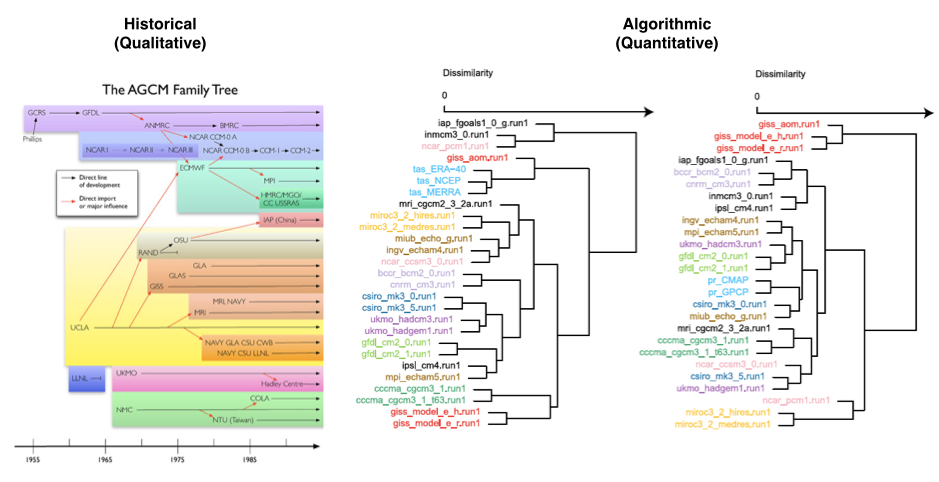
\includegraphics[width=\textwidth]{Model}
\caption{Two previous genealogical studies in climate science. (Left: (Edwards, 2010); Right: (Knutti et al., 2013))}
\label{fig:LABEL2}
\end{figure}

Our work on an ICOADS genealogy somewhat diverges from these previous studies in that
we aren't making an evolutionary metaphor or analogy, we are directly
borrowing techniques and software from phylogenetics \citep{page2009molecular} in trying to
quantify and subsequently visualize the relatedness of climate data.
Part of the ambition in taking a biological approach to studying
material aspects of ICOADS was to leverage the explanations and theories
that this field offers for cooperation \citep{nowak2006five}. If ICOADS data
products did have a traceable evolution then it might be possible to use
concepts like kin selection, fitness, group selection, and reciprocity
(direct, indirect and network) to shed light on how the data have been
reused, shared, developed, or refined. We
were not trying to create a direct mapping between biotic
reproduction and abiotic data reuse, but we were taking seriously the
ecological metaphor that is often invoked in discussing the complexity
of software / data intensive enterprises \citep{weber2013niche}\\

\textbf{Methods} \\
To trace the genealogy of ICOADS, we searched for and
harvested metadata records from NASA's Global Change Master Directory
(GCMD) using the ISO 19115 standard. We used queries related to ICOADS
such as ``International Comprehensive Ocean and Atmosphere Dataset'' or
``I.C.O.A.D.S'' to locate as many ICOADS records as possible. In total,
we discovered 99 records, of which only 23 represented different
versions or subsets of the ICOADS project. This means that the remaining
(n =76 ) records represented derivatives or offspring of ICOADS.\\

We then identified properties (or characteristics) of climate datasets
which we thought would be unique and important to signifying change from
one generation of ICOADS data to the next. This included things like
format, encoding, or the available parameters of the data set. We then
extracted fields containing these properties from the metadata
records. The fields harvested included: Entry Title, Entry ID, Summary,
Geographic Coverage, Start Date, End Date, Geographic Resolution,
Temporal Resolution, Scientific Keywords (often dataset parameters),
Geographic Keywords, Sources (platform of data collection), and
Instruments.\\

Next, we converted each field into binary codes for ``presence'' or
absence'' of individual keywords (Figure 1.2). In some cases we coded
additional ``presence'' or ``absence'' of characters based on the free
text summaries of the records (for instance, in some cases, resolution
was stated in the free text ``Summary'' field but not the ``Geographic
Resolution'' field).\\

\begin{figure}[t]
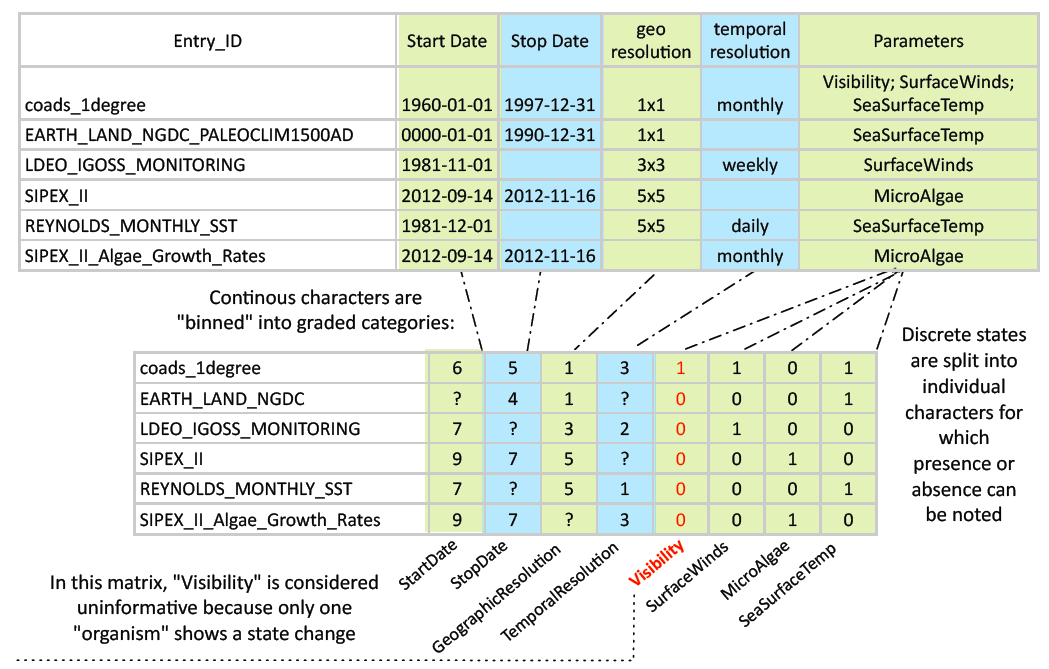
\includegraphics[width=\textwidth]{ICOADS_Coding}
\caption{The migration of metadata records (top) to a character matrix (bottom). Uninformative characters like the
one shown (“Visibility”) cannot show extensive relatedness between groups of "organisms" (Adapted from Thomer and Weber, 2014)}
\label{fig:my_label}
\end{figure}


With the coded data, we then produced a maximum likelihood (ML) tree
\citep{felsenstein1981evolutionary}, by utilizing a statistical model specifically
designed for use with morphological, or presence/absence data \citep{lewis2001likelihood}. Again, the assumption that we were making in this process is that
significant properties or characteristics of the metadata records could
be clustered - such that data products that shared similar traits could
be grouped together in the same way that similar species are grouped
together in a phylogenetic analysis (for a complete discussion of this
work see  \cite{thomer2014phylo}; Weber, Thomer, and Worley, 2014).\\

Our preliminary efforts were successful in creating a tree that
chronologically resembled the release schedule of ICOADS (e.g.~the root
node was the earliest release of ICOADS and furthest nodes were latest
releases). To evaluate the accuracy of this work, we presented a poster
at the Fourth JCOMM Workshop on Advances in Marine Climatology, which is
a major event in the ICOADS community. We asked participants to annotate
our tree, and give us feedback on:\\

\begin{enumerate}
\def\labelenumi{\arabic{enumi}.}
\itemsep1pt\parskip0pt\parsep0pt
\item
  The accuracy of the clustering of related datasets, and
\item
  Datasets related to or derived by ICOADS that were missing from our
  tree.
\end{enumerate}

\textbf{Outcomes}\\ 
The feedback from the ICOADS community verified the
accuracy of our work. In particular, many scientists recognized the data
products that were clustered based on related features, such as
derivative sea-surface temperature (SST) or arctic sea ice data
products. However, a number of curators from other data repositories were able to identify missing datasets, and logical  relationships between clusters that were not well represented by the tree structure (See Figure 1.3 for annotations).\\

\begin{figure}
\centering
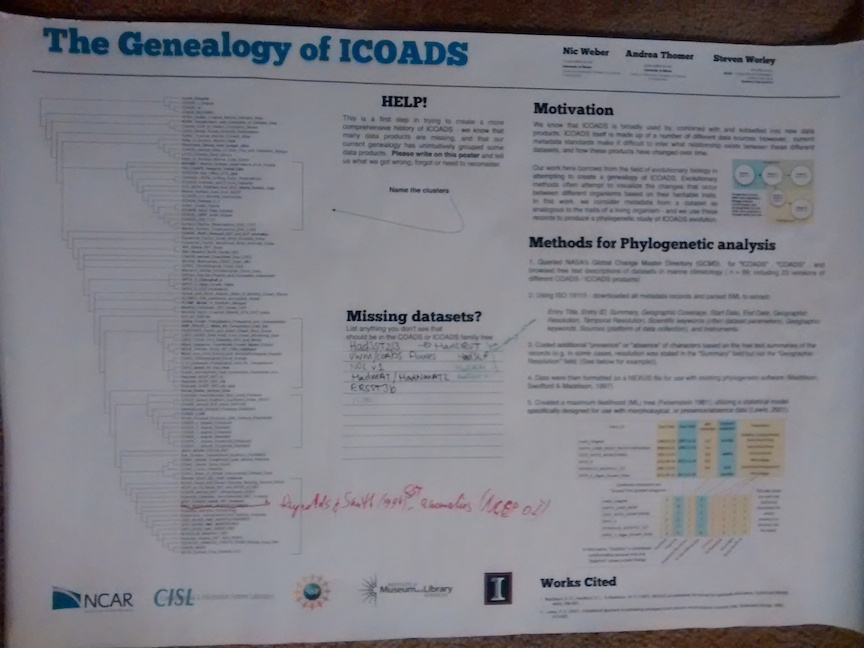
\includegraphics[width=\textwidth]{gen}
\caption{Annotations from the ICOADS community on initial draft of ICOADS genealogy}
\label{fig:my_label}
\end{figure}


Many participants also noted that while the phylogenetic tree showed a
valid evolution of the data products, the title genealogy was misleading
for ICOADS as a project. Notably, the ICOADS community has evolved over
time to include international partners that brought different needs,
data, software, and skills to the collaboration. For instance, our tree
showed that certain data products from the UK's Met Office Hadley
derived from ICOADS only very recently, but we couldn't explain that
this happened because of a governance change at Hadley that allowed for
the data to be obtained by NOAA during this time period \citep{parker2004second}.\\

In short we succeeded in quantitatively representing the evolution of
ICOADS data products, but our work revealed a number of interesting questions
to be asked about how external pressures, technological change, and
political events shaped the evolution of ICOADS as a project, beyond its
material resources. These insights led to a second set of research
questions:\\

\textbf{RQ2}: How has ICOADS, as a  project with particular
governance arrangements, evolved in response to external pressures from
funding agencies, the politicization of climate related research,
and rapid technological change?\\

\section{Policy Relevant eScience Studies}\\

In the next chapter I define concepts and identify findings from existing literature that are relevant to my first two research questions. However, a major gap that I recognized in this literature is policy relevant eScience research. By this I mean social scientist who have studied the use, development, or deployment of a technology and the consequences or affordances  of that work based on its relationship to federal policies - either surrounding the practice, funding, or management of science and technology applications. This seems a strange gap because many social science studies in eScience settings begin a research paper (journal article, conference proceeding, etc.) by arguing for the relevance of their topic via federal policy documents, such as the the 'Blue-Ribbon Advisory Panel on Cyberinfrastructure' report \citep{atkins2002revol}. Too often these studies fail to connect the conclusions and findings of their work back to this arena \citep{jackson2013cscw}. As a result much of science and technology policy at a federal level struggles to appreciate the complexity of developing and sustaining eScience applications \citep{katzframework}. If part of the argument being made in eScience studies is that  high levels of federal funding investment are an indicator of their importance then it should follow that the work in studying these settings is also of significance to funding agencies. To put it another way, if science policy makes a topic relevant to study then the results of studying that topic should also be relevant to science policy.\\ 

So, why have socio-economic and socio-ecologial studies of sustainability been successful at studying institutions while sociotechnical studies have thus far failed to have a strong impact on science policy? Largely because the other domains have developed diagnostic tools and analytical frameworks that allow disparate, unique case studies to be compared to one another so that meaningful design principles can emerge \citep{ostrom2007diagnostic}.\\

This leads to my third research question:\\

\begin{quote}
\textbf{RQ3}: How can analytical frameworks successful for studying
collective action problems in other domains be modified for
sociotechnical settings where issues of sustainability, cooperation and
shared resource management are diverse and shifting over time?
\end{quote}

The major contribution of this dissertation is a framework that will facilitate the integration and combination of different methods to investigate complex, systems-based problems as they relate to the sustainability of cooperative eScience projects. This will be done by incorporating relevant categories from existing sustainability frameworks, and systems theory. In the next chapter, I argue why this is needed from a conceptual standpoint, and how the work of institutional scholars can help address current shortcomings in bringing existing eScience studies to bear on science and technology issues. 

\chapter{}

\emph{In chapter two I review literature relevant
to a study of cooperation and collective action in an eScience setting.  In each section I define a concept, review previous work
or background of the concept, and then explain the relevance to ICOADS.}

\section{Peer production}

Organizing work on the internet found early success in free libre open source software
(FLOSS) projects like Linux, FetchMail, PERL, and Apache. Organizational scholars \citep{lakhani2003open, lakhani2005hackers} and economists \citep{lerner2002some, hars2001working} both  marveled at the success of FLOSS projects, and their ability  solve traditional resource allocation problems outside of either a firm (hierarchy) or a marketplace setting. In this sense, FLOSS projects contradicted many basic economic assumptions about organizing, divisions of labor, and intellectual property \citep[e.g.][]{coase1937nature, schumpeter1942capitalism, becker1976economic}. A finding often repeated from these early studies of FLOSS development was not that participants were a new breed of altruistic worker, but that organizing projects via networked technologies allows for a more diverse set of interests, preferences, and motivations to emerge than was accommodated by traditional synchronous,  face to face venues \citep{benkler2006commons}.\\

In his broad study of open-source software development and the unique
legal and economic arrangements that were created by individuals
coordinating projects via the Internet, Yochai Benkler described this
new mode of organizing as peer production:

\begin{quote}
\ldots{}a form of open creation and sharing performed by groups online
that: set and execute goals in a decentralized manner; harness a diverse
range of participant motivations, particularly non-monetary motivations;
and separate governance and management relations from exclusive forms of
property and relational contracts (i.e., projects are governed as open
commons or common property regimes and organizational governance
utilizes combinations of participatory, meritocratic and charismatic,
rather than proprietary or contractual, models)" \citeyearpar{benkler2013peer}.
\end{quote}

This original definition led to further qualifications of how peer production is accomplished, such as a
commons-based model that is, ``radically decentralized, collaborative,
and non-proprietary; based on sharing resources and outputs among widely
distributed, loosely connected individuals who cooperate with each other
without relying on either market signals or managerial commands'' \citep[p. 61]{benkler2006wealth}.\\

Haythornthwaite later drew a distinction between heavyweight and lightweight models of  peer production:

\begin{itemize}
\item
  In a lightweight model of peer production, such as crowdsourcing, many
  loosely connected individuals contribute their effort to accomplishing small,
  well-defined and highly coordinated tasks. 
\item
  In a heavyweight model strongly connected and highly committed
  members, such as those in a virtual organization (VO), perform loosely
  coordinated tasks, and their contributions are accepted based on
  quality control mechanisms like peer review \citeyearpar{haythornthwaite2009crowds}.
\end{itemize}

\subsection*{Second Order Peer Production}
For social scientists, part of the attraction to studying peer production systems
is the \emph{apparent} egalitarian nature of ``communal information goods'' \citep[as quoted in\cite{shaw2014laboratories}]{fulk1996connective}. Many of the FLOSS successes listed above have created democratic organizations that have had transformative and
lasting success in industries that are traditionally dominated by
private firms (i.e.~Firefox web browsers, Linux and Android operating
system, etc.). But, after the initial novelty of peer production was described \citep{benkler2006wealth}, a series of what might be called second order peer production studies looked closer at these institutions and the context of their success. These studies
used quantitative methods to show, for instance, that most FLOSS projects
are the work of a few key individuals making large contributions \citep{shah2006motivation}; by most measures these individuals are highly uncooperative \citep{hill2009official}; that Wikipedia is a single success in what were
many similar wiki-based encyclopedia projects that failed  \citep{kittur2008harnessing, ortega2009wikipedia}; and that the assumed democracy of wiki-based projects actually resembles an oligarchy when studied over time \citep{shaw2014laboratories}.\\

Most recently, organizational scholars have started to turn
their attention from what has made the Apaches and Wikipedias of peer
production successful towards what has caused similarly structured
projects to fail \citep{shaw2014laboratories}. This is a familiar turn that can be observed in early CSCW groupware research that first focused on successes \citep{winograd1986language} and later on what caused their failures
\citep{grudin1988cscw}. This pattern is also recognizable in fields like
innovation studies where Michael Porter first explained a firm's success
through ``competitive advantage'' \citeyearpar{porter1987competitive}, while his protege Clayton M.
Christensen later explained a firm's failure through a theory of disruption \citeyearpar{christensen2006ongoing}.\\

\subsection*{Peer Production in ICOADS}

Many of the features from Benkler's original definition of peer production, such as 'setting and executing goals in a decentralized way' and 'the separation of governance models from management relations,' were simultaneously described in interdisciplinary research settings \citep{palmer2001work}. Other works on scientific collaboration  show these same features, and took place far before adoption of networked technologies like the Internet \citep{galison1997image}. But, evidence of a shift in how work is accomplished in interdisciplinary settings can be seen, for instance, in the approach to developing earth systems models which evolved from the centrally organized effort of a single institution, to open-source ``community models'' that couple many different physical system models developed by loosely connected, highly cooperative research institutions around the world -
very much following a commons-based peer production as described
above  \citep{edwards2010vast, voinov2010community}.\\

For ICOADS, much of the work that led to the initial development of a
``comprehensive'' dataset was through the open sharing of data between
groups at different institutions, who set and executed goals in a
decentralized way, and they did so with little to no external
organizing pressure \citep{slutz1985comprehensive}. As the ICOADS project grew,
it became more diverse and more international. This allowed for developers who
were motivated by the need to fill a gap in the data used to calculate
climate change indexes to contribute in a loosely coordinated fashion
that strongly resembles heavyweight peer production models.\\

\section{Open science}

In short, open science is a set of governance structures that provides a
``specific non-market reward system to solve a number of resource
allocation problems'' \citep{david2003economic}. This alternative to privatization
applies to both the distribution and production of scientific information as an
economic and public good. Open science is the theoretical foundation
that allows commons-based property regimes in science to supplant the often private
or government controlled rights to access that dominate other spheres of
economic activity \citep{david2004understanding}.\\

\subsection*{Open Science and Research Impact}

A formidable challenge to adopting open science practices is that a non-market based reward system has yet to fully emerge. This is especially limiting in the academic environment where the promotion and tenure of scientists (and technologists) is still largely based on individual, supposedly merit-based evaluations. So, although there are
many emergent practices of openly sharing and pooling resources in domains that rely on open
science \citep{willinsky2005unacknowledged, stodden2010open},
use of traditional market-like mechanisms for measuring performance or impact (e.g. bibliometrics, grant funding levels, etc.) limits their broader adoption.  Many
alternative scientometric techniques are promoted as a
remedy to the limitations of traditional measures of impact \citep{bollen2005toward, priem2012altmetrics, piwowar2013altmetrics }, but as I demonstrated in chapter one,
the utility of metric based approaches to understanding re-use,
sharing, or policy interventions in an open science community are
greatly limited by the quality, scope, and reliability of data for these
types of analysis.\\

This also creates a bit of a conundrum because in many ways alternative measures of impact are made possible by practices of open science, but the sharing and pooling of resources across traditional boundaries of intellectual
property rights and ownership also renders many quantitative
approaches from scientometrics ineffective in measuring the impact of
any one resource, organization, or project. The task of what Partha and David have previously called a `new economics of science' is to better inform policy making through a combination of economic calculations of value according to the efficient allocation of informational resources, with the structural functionalism of sociology, which investigates reward systems, institutions and behavioral norms in knowledge production \citeyearpar[p. 487]{partha1994toward}. They argue that in combining these two traditions, science and technology policy might better realize the value proposition of open science, which is impossible to fully grasp through simple measures like a pure cost benefit function or scientometric measure like the h-index. The work presented in this dissertation takes seriously the combination of these two traditions in assigning values to open science work, but (for reasons discussed below) I move away from the structural functionalist tradition of Merton, locating a more useful form of functionalism in the work of Elinor Ostrom's institutional studies. 

\subsection*{Open Science in ICOADS}

ICOADS was originally assembled through cooperative exchanges between NOAA, NCAR, and national
maritime archives around the world. The early literature describing this work often states
that the open accessibility and free cost of ICOADS data was meant to reflect
this spirit of cooperation \citep{slutz1985comprehensive}. A publication
describing the latest release of ICOADS (2.5) reaffirms this in stating,
``This is an open community and new participants are welcomed. As part
of this involvement, we hope that nations and organisations taking and
holding marine surface observations can continue to examine the pathways
by which their information is shared'' \citep{woodruff2011icoads}. Part of the challenge to be addressed in my case study of ICOADS is how to combine observations of effective resource allocations made during the DUI study, with the functional aspects of the ICOADS community that was emphasized during the genealogy study.\\

\section{Collective action}

Collective action can be defined simply as, ``action taken by multiple
people in pursuit of the same goal or collective good''
\citep{oliver1993critical}. As Parth and David noted in their discussion
of a new economics of science \citeyear{partha1994toward}, the early collective action work of
sociologist Robert K. Merton has been influential to scholars trying to
establish an intellectual framework for open science.\\

In brief,  Merton and colleagues were not interested in the content of scientific
knowledge, but instead the norms, values and incentives that a culture
uses to guard against change, or adapt and
evolve to external pressures over time \citep{hess1997science}. Merton's work in sociology was therefore concerned with, ``\ldots{}the
cultural structure of science, that is with one limited aspect of
science as an institution\ldots{}.we shall consider, not the methods of
science, but the mores with which they are hedged about'' \citeyearpar[p. 268]{merton1973sociology}.\\

A key point of
Merton's work -- and one that is highly contested in contemporary
Science and Technology Studies -- is that science was positioned as a
neutral domain of knowledge production. This privileged status of knowledge was achieved by what Merton claims to be an objective "disinterestedness" of a scientist \citeyear{merton1973sociology}. From this perspective, the study of social functions in science were to be observed by objective
consequences of activities; that is,  social functions could not be explained
interpretively through subjective dispositions (motivation, incentives,
reward structures) \citeyearpar[Ch. 13]{merton1973sociology}.\\

This legacy of Merton's functionalism is evident in much of Elinor
Ostrom's work on commons and shared governance arrangements \citeyear{ostrom1990governing}. Where the two traditions differ is that Ostrom
rejected Merton's notion of subjective and objective consequences of
social functions, as well as the idea that any particular
domain held a privileged status with respect
to rationality or neutrality. Further, in place of society, Ostrom and
colleagues were concerned with smaller functional structures; asking
instead how an \emph{institution} functioned in light of activities that
promote or interfere with the maintenance of a shared physical resource  \citep{aligica2009challenging}. In this context,
institutions are to be understood as, ``enduring regularities of human
action in situations structured by rules, norms, and shared strategies,
as well as by the physical world. The rules, norms, and shared
strategies are constituted and reconstituted by human interaction in
frequently occurring or repetitive situations'' \citep[p. 582]{crawford1995grammar}. \\

Ostrom's unique approach to functionalism relies upon
understanding how purposefully organized groups of people use, share, or
pool resources over time, and to what extent the success of these
arrangements are governed by informal and formal rules, where rles are defined as, ``prescriptions that forbid, permit, or require
some action or outcome and the sanctions authorized if the rules are not
followed''  \citep[as quoted in \cite{imperial2005taking}]{crawford1995grammar}.  When institutional scholars, following Ostrom's work, dismissed the idea of ``objectivity''
they replaced Merton's social functions with intended and unintended
consequences, using the verbiage of economics to imply that there are
positive or negative externalities (sometimes called spillovers) that
result from collective action. What Ostrom and colleagues attempted to
understand through their study of rules and shared resources was how
externalities were designed for and managed in institutions for
collective action. A concern for both the functioning of institutions
over time and the material aspects of collective action makes Ostrom's
work especially relevant to contemporary studies of eScience
sustainability.\\

\subsection*{Collective Action in eScience}

Studying collective action in scientific settings, whether it is
informed by the work of Merton, Ostrom, or Parth and David's new
economics of science, is really to ask a set of questions about
cooperation that is central to all of social science, ``How do fallible
humans come together, create communities and organizations, and make
decisions and rules in order to sustain a resource or achieve a desired
outcome?'' \citep[p. 42]{hess2007understanding}. Information science has long
been concerned with the material aspects of this question \citep{bates1999invisible}, including the
discoverability, use and preservation of research products that result
from collective actions in science. These traditional
problems are addressed in this proposal by drawing upon theories of
human organization that attempt to explain how ``a group of principals
can organize themselves voluntarily to retain the residuals of their own
efforts'' \citep[p.25]{ostrom1990governing}. I am particularly interested in how it is
that individuals and institutions with overlapping research agendas are
able to resolve conflicts, and coordinate their actions to
successfully cooperate over long periods of time, with very little
government intervention, oversight, and most recently, funding.\\

\subsection*{Collective Action in ICOADS}

In collective action scenarios, like ICOADS, where the performance or
sequencing of activities greatly overlap there is the potential for
conflict to arise in how best to achieve a shared goal. Mechanisms for
identifying, and solving conflicts between different individuals then
becomes paramount to the effective functioning of any given organization
that depends upon some form of collective action - and this is
especially important to those cooperatives that operate through
computer mediated communications \citep{easterbrook1993survey}. This is not
to say that conflict is not an important aspect of a highly functioning
collaborative project; contemporary studies of conflict show that, for
instance, resolving disputes over internet relay chat (IRC) allowed the
distributed FLOSS project GNU Enterprise (GNUe) to codify unspoken
norms, and create an archive of decision-making that they could refer to
in future disputes \citep[similar observations are made in \citep{coleman2005three}]{elliott2003free} .\\

ICOADS relies on many forms of collective action to curate, develop, or serve its software and data to end users. An especially active area of collective action in ICOADS is related to data quality control and bug reports sent to curators. Part of the value proposition for end users is that although ICOADS data are homogeneous and well described, they are of varying quality and coverage. Understanding limitations in the data such as regions or time periods that suffer from a limited number of observations can be communicated through publications, bug reporting, and email list-servs. Incorporating fixes, or resolving conflicts is often done through a peer-review like process, which makes the "heavyweight" categorization of ICOADS peer production so useful. Further understanding patterns of conflict resolution, and the ways in which the culture of ICOADS functions in these moments is an important aspect of the case study design (described in chapter three). 

\section{Commons}

In open science the alternative to a private intellectual property
regime is a commons-based approach, which provides rules and norms for
the governance of resources that ``require larger scale utilization than
would be efficient in small, individually-owned parcels'' \citep{benkler2011between}. ``Commons'' is also a term used loosely by institutional scholars
and economists to critique the neoclassical model of property ownership
\citep{hess2003ideas}.\\

In a commons, the operational structure allowing for access, use, and
ownership of a shared resource is distributed amongst the stakeholders
of those resources; this can be applied to wholly public goods, or some
combination of intellectual property rights for a group and for individual participants, such as
a common-pool resource. Increasingly, the legal framework of common
property is applied to collections of digital assets that are
collectively produced, managed or funded \citep{hess2007understanding}. A digital environment that distributes work through
peer production needs both an intellectual and a legal framework like
the commons, as it provides ``a coherent alternative model for bringing
economic, social, and ethical concerns into greater alignment. It is
able to talk about the inalienability of certain resources and the value
of protecting community interests. The commons fills a theoretical void
by explaining how significant value can be created and sustained outside
of the market system.'' \citep[p. 27]{bollier2007growth}.\\

Some of the most recognizable forms of commons can be found in the
shared maintenance of natural resources such as Atlantic Cod fisheries
\citep{hutchings1994can,}, Maine's lobster industry \citep{acheson1988lobster},
and livestock grazing pastures \citep{ostrom1999revisiting}. Examples of digital commons include
Wikipedia, collections of cultural material like the Hathi Trust, and
open source software projects like Apache, Linux, and Android \citep{benkler2011penguin, madison2010constructing}\\

A heuristic tool for understanding the nature of any commons arrangement
is to analyze how a shared resource is able to be accessed, and the
rivalry that this access creates amongst its users \citep{ostrom1994rules}. To understand
rivalry we can ask questions like `Is there competition for the
resource? Is the resource finite, or renewable? Can the resources be
simultaneously accessed and owned by two or more individuals?' In the
other dimension, we can ask questions about the excludability of a resource,
such as 'Can potential users of commons be denied access (either by
physical means or on moral grounds)?' Using these two characteristics of
a resource we can situate almost any commons arrangement in the
following matrix:

\begin{figure}
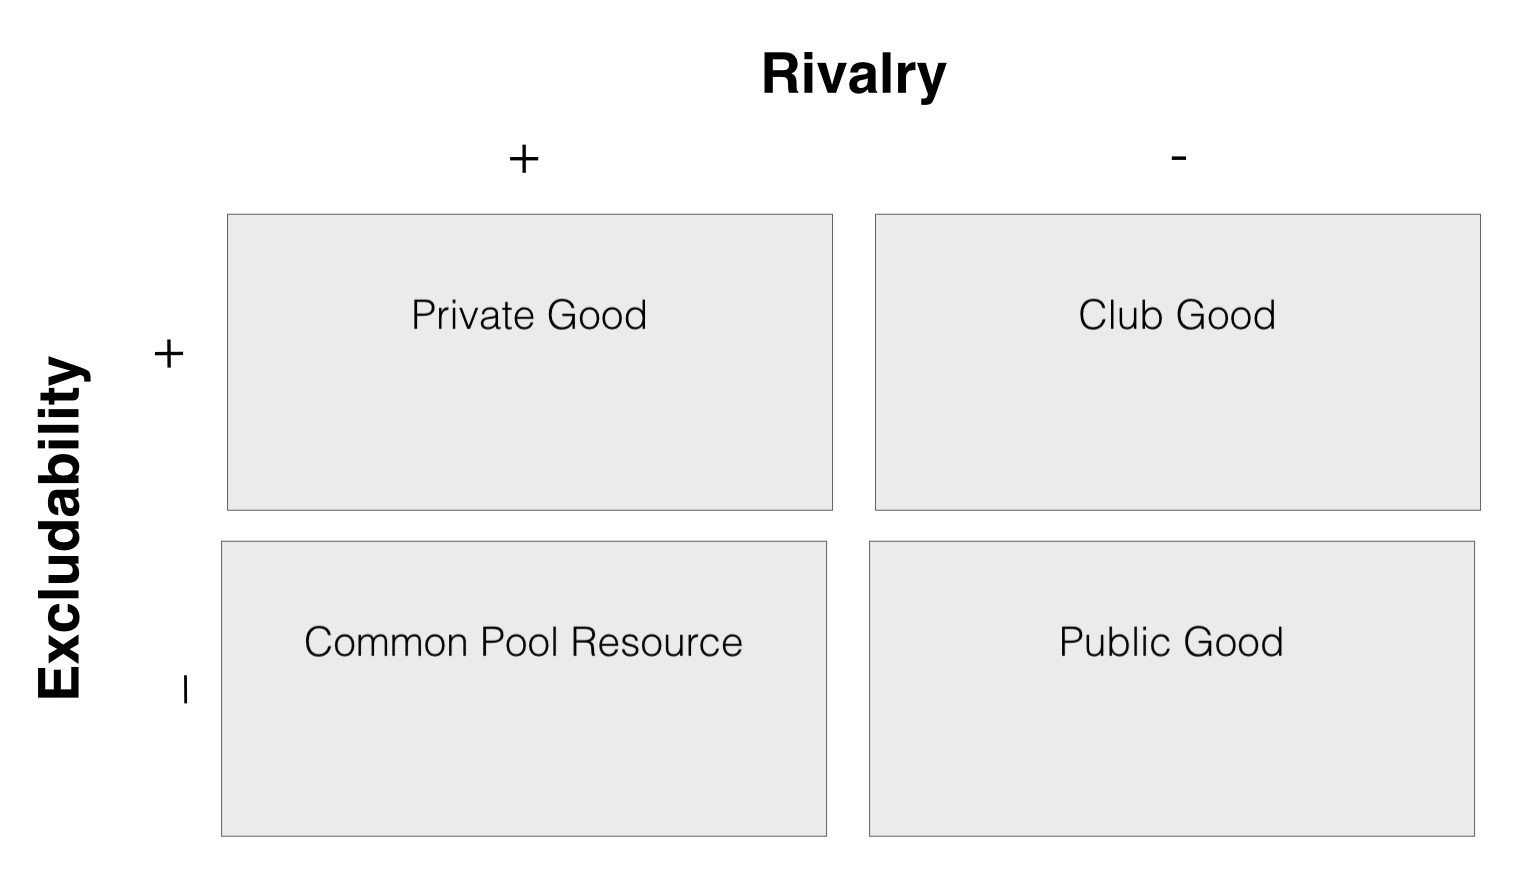
\includegraphics[width=\textwidth]{CommonsMatrix}
\caption{Matrix of commons adapted from \citep[p.7]{ostrom1994rules}}
\label{fig:my_label}
\end{figure}


Elinor Ostrom's early work on common-pool resources and their governance
structures \citeyear{ostrom1990governing} was the foundation for much of the scholarship that is
labeled ``commons'' including concepts that extended or modified her
findings, such as the ``anticommons'' \citep{heller1998tragedy}, ``semicommons'' \citep{smith2000semicommon}, ``creative commons,'' ``contractually reconstructed
commons'' \citep{reichman2003contractually}, ``liberal commons'' \citep{dagan2001liberal}, and the ``culturally constructed commons'' \citep{madison2010constructing}.\\

In this proposal my focus is on public goods, where the management of a
resource or service has low levels of both rivalry and excludability\footnote{Intellectual property laws are meant to encourage the production of
public goods by creating legal barriers to copying,
distributing and sharing these types of materials. Where appropriate I
will discuss intellectual property law, but for the most part I avoid
discussions of formal laws by focusing on public goods which are to
remain in the public sphere, and are therefore governed by informal
rules and community norms.}.
\\

\subsection*{Science Commons}

A science-based commons is simply a ``species of commons dedicated to
scientific data and information'' \citep{contreras2010data}, but this label is
also applicable to the pooling of software, instruments, and computing
resources necessary to effectively conduct research in an open science
environment. Similar to a natural resource system, the pooled goods making
up a science commons are subject to different forms of competition, and
barriers to access. That is to say, data, software and other products of
basic science research play different roles within different evidential
cultures in which they are produced \citep{collins1998meaning}. It follows then
that these products exhibit varying degrees of rivalry and
excludability.\\

Surprisingly, this point is not made more explicit in studies of
eScience resource sharing and pooling. Instead, ``data'' are often
assumed to have high degrees of rivalry, and so are either considered to be a
private good or a common pool resource. For instance, Birnhotlz and
Bietz discuss at length the economic principles of ``rent extraction''
for AIDS researchers who attempt to maximize the return value on their
shared data \citeyearpar{birnholtz2003data}. Birnholtz and Bietz use rent extraction to then
describe design implications for systems that will store, and manage
``scientific data'' more broadly, claiming that these self-interests
should be played upon rather than subverted. Similar treatments of
research data as a private good or common-pool resource can be found in \citeyear{zimmerman2008new}; \citeyear{faniel2010reusing}; and \citeyear{tenopir2011data}. This is not to say that any of these studies are wrong in their
classification of research data as a rivalrous good, but it is to say
generalizing about design requirements or policy implications for
``scientific data'' from the study of particular sub-cultures or
sub-disciplines \emph{is} ineffective. At best, these studies can
provide general findings about sharing and resource pooling for goods
based on their role within certain commons regimes.\\

In a science commons, a distinction between rivalry in access and
rivalry in use is important to clarify. In some sense, two individuals
might both be able to obtain the same set of data from the same commons,
but the very fact that two individuals have the data and have the ability to draw
similar conclusions does not necessary mean that they will. In the case
of ICOADS the ``raw'' nature of marine climatology data creates a need
to further process the data in order to derive any substantive meaning
from it. Therefore, mutual ownership does not in any way lessen the
value of ICOADS data, software, or other resources. Techniques, software and computing time to do that processing is however execptionally rivalrous, and is the source of a great deal of competition amongst the community's participants.\\

\begin{figure}
\centering
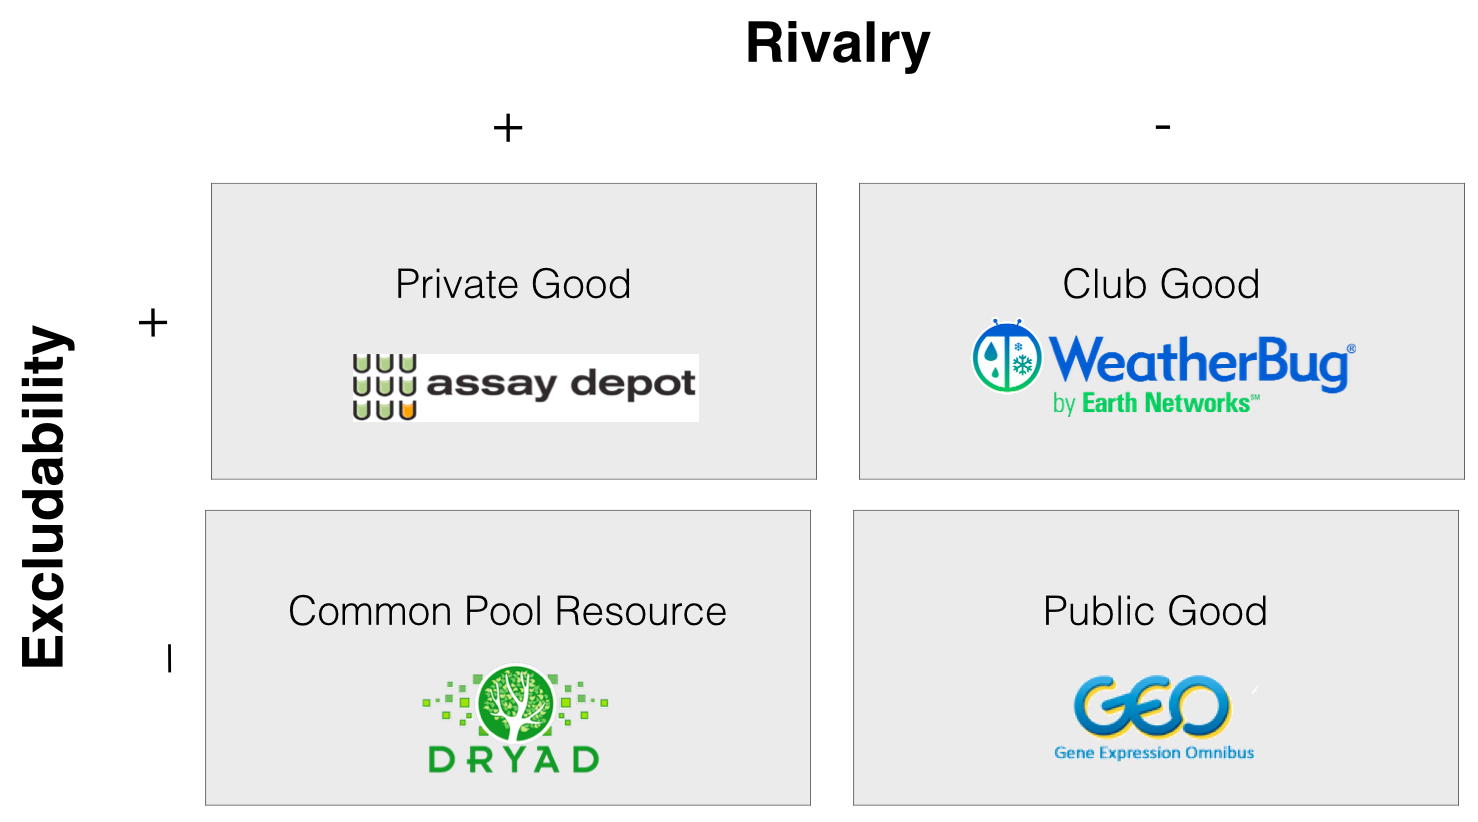
\includegraphics[width=\textwidth]{ScienceCommons}
\caption{Different institutions in the Science Commons according to their rivalry and excludability.}
\label{fig:my_label}
\end{figure}


\subsection*{Science Commons and Public Goods}

Although the idea of a science commons and common-property frameworks
being applied to digital material is a relatively new phenomenon
\citep{arzberger2004promoting,wilbanks2006introduction,contreras2010data} 
scientific knowledge has long been referred to as a
``quasi-public-good'' \citep{fuller1993philosophy}. Callon explains the
economic distinction in saying, ``The qualification of science as a
quasi-public good rather than as a full-fledged public good derives
essentially from the fact that it is to a certain degree
appropriable-whereas in standard theory a true public good has to be
completely inappropriable'' \citep[p. 400]{callon1994science}. Increasingly, economists
argue for scientific works funded through government subsidies
(e.g.~journal publications, data, models etc.) to be considered
quasi-public-goods for two reasons:

\begin{enumerate}
\def\labelenumi{\arabic{enumi}.}
\item
  Scientific knowledge has certain intrinsic characteristics that make
  it difficult to exclude access to, and even more difficult to directly
  commodify. Material products of this enterprise, such as data or
  software, are the informational carriers of that knowledge, and so
  restricting use or access is equatable to creating artificial barriers
  to facts and knowledge\footnote{This argument very much turns on legal jurisdictions \citep[see][for USA precedence]{copyright1998us} }.
\item
  Market mechanisms cause businesses to under-invest in basic science
  research, therefore the government subsidy of this work marks it as a
  good which is publicly funded and requires collective access. 
  \citep{callon1994science}.
\end{enumerate}

The final two sections of this chapter address the problem of free riding that often
emerges in public goods settings. This literature provides important
background for studying the evolution of commons arrangements.\\

\section{Tragedy of the Commons, Free Riders \& Cooperation}

Garret Hardin first coined the phrase ``tragedy of the commons'' to
describe problems of overpopulation \citeyear{hardin1968tragedy}. Hardin's argument depends on
a hypothetical collective action dilemma from an open grazing pasture.
As each individual is concerned with only her/his own well being they
are motivated to increase the size of their herd. With no incentive to
limit this growth, the size of all herds will swell while the grazing
spaces remain the same. This in turn leads to the overgrazing and
destruction of the common space:

\begin{quote}
Therein is the tragedy. Each man is locked into a system that compels
him to increase his herd without limit-in a world that is limited. Ruin
is the destination toward which all men rush, each pursuing his own best
interest in a society that believes in the freedom of the commons.
Freedom in a commons brings ruin to all. \citep[p. 1244]{hardin1968tragedy}.
\end{quote}

The tragedy of the commons is an example of what economists have long
referred to as the free rider problem. The logic of this idea is
explained by Ostrom, ``Whenever one person cannot be excluded from the
benefits that others provide, each person is motivated not to contribute
to the joint effort, but to free-ride on the efforts of others. If all
participants choose to free-ride, the collective benefit will not be
produced. The temptation to free-ride, however, may dominate the
decision process and thus all will end up where no one wanted to be''
\citep[p. 6]{ostrom1990governing}. Free riding becomes possible when the total benefits
from collective action are not a direct result of any one individual's
actions. When a group reaches a size where contribution to a common pool
becomes difficult to track and group membership is easy to obtain, then
the phenomena of free riding can emerge: individual actors may consume
or use more than they contribute.\\

The size function of the free rider problem is often positioned as the
most important variable leading to a ``tragedy of the commons.'' Mancur
Olson's early economic work on this problem presented the following
thesis:

``Unless the number of individuals in a group is quite small, or unless
there is coercion or some other special device to make individuals act
in their common interest, rational, self-interested individuals will not
act to achieve their common or group interests.'' \citeyearpar[p. 2]{olson1965logic}

Since Olson's writing, Elinor Ostrom and a number of other influential
political scientists have demonstrated that while group size is an
important variable for sustainable commons arrangements, the devil is in
the details; groups large and small often succeed in solving
collective action problems through self-governance, and whats more, the
logic behind such assumptions about the failure of these arrangements often
does not hold up in laboratory simulations, nor real-life scenarios
\citep[for an overview of the long history of this refutation by Ostrom see(][]{aligica2009challenging}.\\

In laboratory settings, Fehr and Schmidt conducted some of the first collective action studies on reciprocity, finding that  ``economic environment determines whether the fair types or
the selfish types dominate equilibrium behavior.'' \citeyear[p. 817]{fehr1999theory} or
put another way, ``contextual factors affect the rate of contribution to
public goods'' \citep{ostrom2005}, where contextual factors of the economic
environment can include the number of players involved, the resources
exchanged, and the framing of a scenario. In the latter example, a
number of studies have focused on the importance of contextual framing
for cooperation to emerge, finding that when participants are told they
are playing a ``Wall Street'' game they produce less cooperative
outcomes, but when the same variables are tested using the framing of a
``community'' game, cooperation is more likely to emerge and be
sustained over time \citep{liberman2004name}.\\

\begin{table}[h]
\begin{tabular}{lll}
             & \textbf{I Cooperate} & \textbf{I Defect} \\
\textbf{You Cooperate} & b-c         & -c        \\
\textbf{You Defect}    & b           & 0       
\end{tabular}
\end{table}

\textit{The range of a prisoners dilemma payoff, where b>c>0}\\

In his seminal work on the evolution of cooperation, Axelrod first develop probabilistic models to solve the "prisnoers dillema" game. Based on the likelihood of future interaction he was able to show how, "cooperation based on reciprocity can get started in an asocial world, can thrive while interacting with a wide range of other strategies, and can resist invasion once fully established" \citep{axelrod1981evolution}. His later work hosted tournaments to solve the ``prisoners dilemma'' game  through algorithms where the most simple strategies were the most effective in creating
sustainable cooperation (such as a tit-for-tat reciprocity), and this repeated his early findings that
cooperation emerged largely as a function of the likelihood that players would
interact in future rounds \citeyear{axelrod2006evolution}. In more recent studies using public
goods games (which simulate simple decisions about collective action
problems similar to the prisoners dilemma) researchers have focused
on how social diversity enables both the emergence of cooperation \citep[for a thorough overview see][]{perc2010coevolutionary}. Many of these studies manipulate a single variable in the game to
produce results which directly counter the inevitability of free riding
as argued by Olson and Hardin. For instance, recent work shows that
contributions to a public pool are more consistent in groups that are
socially diverse ( by race, gender, age, etc. \citeyearpar{santos2008social}), and that cooperators and defectors can
successfully coexist in public goods games where population density is
high if the density remains stable \citep{hauert2006evolutionary}.\\

The emergence of cooperation in collective action dilemmas has also been
studied widely using observational or field-based social science
methods. In the early 1980's Acheson studied lobster fisheries in Maine,
showing that the temptation to poach or over-harvest lobsters was
remedied by a series of nested rules. In this setting some rules were established by gaming and
wildlife commissions at the state level, and others at the community
(dock) level where ``lobster gangs'' would enforce social norms through
physical intimidation and punishment \citep{acheson1988lobster}. During this same
period, Ostrom studied long-enduring Spanish Huertas - fertile areas of
farm and garden land along riversides- showing that a variety of
governance structures could produce highly cooperative outcomes over
long periods of time. Ostrom's work focused on how physical attributes
of a resource system impacted governance structures. Her work showed
that these commons were often sustained through a polycentric\footnote{Polycentricity is rarely discussed outside of political science, but I believe this is a concept that can be exceptionally useful in understanding the functioning of ICOADS and the rules and norms of its governance. Borgman has referred to the overlap in various rules, cultures and policies that impact data sharing as a "conundrum" \citeyear{borgman2012conundrum}.  The nested rules that apply to ICOADS stakeholders, and how the community adjusts (or does not adjust) to those overlapping rules is a dilemma which polycentric governance theory was meant to help explain.}
governance system where, like Acheson's lobster fisheries, informal
rules were nested within formal local and state laws. The huertas
offered a particularly valuable look at the commons phenomenon as these
governance systems have been negotiated and renegotiated over a five
hundred year period \citep{ostrom1990governing}. Many studies followed Ostrom's
seminal work on common-pool resources, some refined the nuances of her
design principles (discussed in detail in Chapter 3), others extended
her work to socio-economic and socio-ecological resource systems \citep[,for a thorough overview]{folke2005adaptive, young2006globalization, ostrom2009understanding,}\\ 

Field based research on free riding in commons that are made up of
digital resources (including virtual, knowledge, creative, or scientific
commons) are rare, but not without precedence. Early work on
collaboratories in CSCW produced the idea of a ``virtual commons''
applied to Usenet - a distributed discussion forum popular on the Internet in the late 1990's. In this work, Kollock and
Smith use the design principles generated by Ostrom \citeyear{ostrom1990governing} to describe
how both free riding and cooperation are made easier in computer
mediated communication systems, with the effect being a more volatile
and dynamic environment for collective action problems to be solved \citeyear{kollock1996managing}\\

A majority of digital commons literature is focused on just two settings
(FLOSS and Wikpiedia), but the results from this work are highly
valuable for understanding the complexity of the free rider problem in
online collaborations more generally. In the FLOSS literature on
commons, von Hippel and Krogh studied participation in OSS projects
using a case study methodology, noting how free riders were identified
and outed in early OSS projects like Fetchmail and Apache \citeyear{hippel2003open}. One of their
main conclusions is tha:t

\begin{quote}
The central deviation we believe that open source
software projects display with respect to the assumptions about
incentives embedded in the private investment and the collective action
models of innovation is that contributions to open source software
development are not pure public goods --they have significant private
elements even after the contribution has been freely revealed  \citep[p. 16]{hippel2003open}. 
\end{quote}

In other words, traditional notions of free riding in public
goods regimes aren't wholly applicable to the OSS environment, because
the spillover (externalities) of participating in the production of the
software is where novel sources of value can be located.
So even if the software is a pure public good the value proposition of
an OSS project is a blend of private and public benefits.\\ 

Much of the early work on Wikipedia as a commons platform focused on the design of a governance model that could
simultaneously attract new participants and sustain existing
contributors \citep[i.e.][]{nov2007motivates}. Interestingly, free riding on Wikipedia is assumed to be pervasive because there are many more visitors
(readers) of the site than there are registered or active contributors
(editors). Antin and Cheshire's work shows that a majority of readers
have incomplete information about how to edit articles, and low
confidence in their ability to correctly use MediaWiki editing software
(\citeyear{antin2010readers}). They conclude that the idea of free riding, in the sense that
readers are taking advantage of others work without reciprocating, is
more nuanced in the Wikipedia environment. From a design standpoint they
argue that the task is not in motivating readers to edit immediately,
but in finding intermediate steps for participation such as viewing page-history
 or talk-pages to become familiar with the culture of editing content on wikipedia.\\

This is a nuanced, but important point for the proposed case study; there are many
more users of ICOADS than there are contributors. ICOADS has recently
introduced new ways for users to report errors and share data \citep{smith2014icoads}. Antin and Cheshire's work provides a helpful example of how to observe participation, contribution, and variations of the the free
rider beyond the level of a user's directly measurable participation.\\

\subsection*{ICOADS Context}

This dissertation focuses on a culture that produces, uses, and
develops resources that are quasi-public-goods because they are managed
with relatively low degrees of exclusivity (i.e.~not many people can be
excluded from obtaining the software or data) and as a result of their
digital form they are not subject to a high degree of rivalry (i.e.~your
having a copy of this dataset does not preclude my having a copy). What
makes ICOADS a unique and highly important case for understanding the
future evolution of institutions for collective action is that the
management of these resources as public goods is not regulated by a federal
government mandate, nor is it a response to some marketplace pricing
signal. ICOADS is a self organizing commons that has persisted for many
years through arranging its production in a commons-based peer
production model. However, ICOADS is also facing a funding shortage, and will face a
number of obstacles in sustaining its commons arrangement in the future.
A substantive question to be addressed in this research is how ICOADS
continues to solve resource allocation problems necessary to sustain an
open-science, commons-based model of peer production.\\ 

\chapter{}

\subsection*{Introduction}

\emph{In chapter three I first describe a range of research methods that
can be used to study peer-produced commons, collective action, and
sustainability. I begin first by explaining how this work will overcome
limitations with the case study approach. I then describe the design and
procedure for a case study of ICOADS, and how it will be used to test a
proposed framework. At the end of this chapter, I describe the overall contribution of this research, and a
schedule of completion.}\\

\section{Empirical Social Science}

Conducting empirical research in the social sciences is often a
trade-off between some combination of available time, money, skills, and
material resources - each presenting a choice between one way of collecting or analyzing data and a number of
alternatives. Generically, we can situate trade-offs between data
collection and analysis in a two dimensional matrix; in one dimension we
can place the choice of an empirical research method, and in another
dimension we can place the use of a theoretical descriptive technique.\\

\begin{figure}
\centering
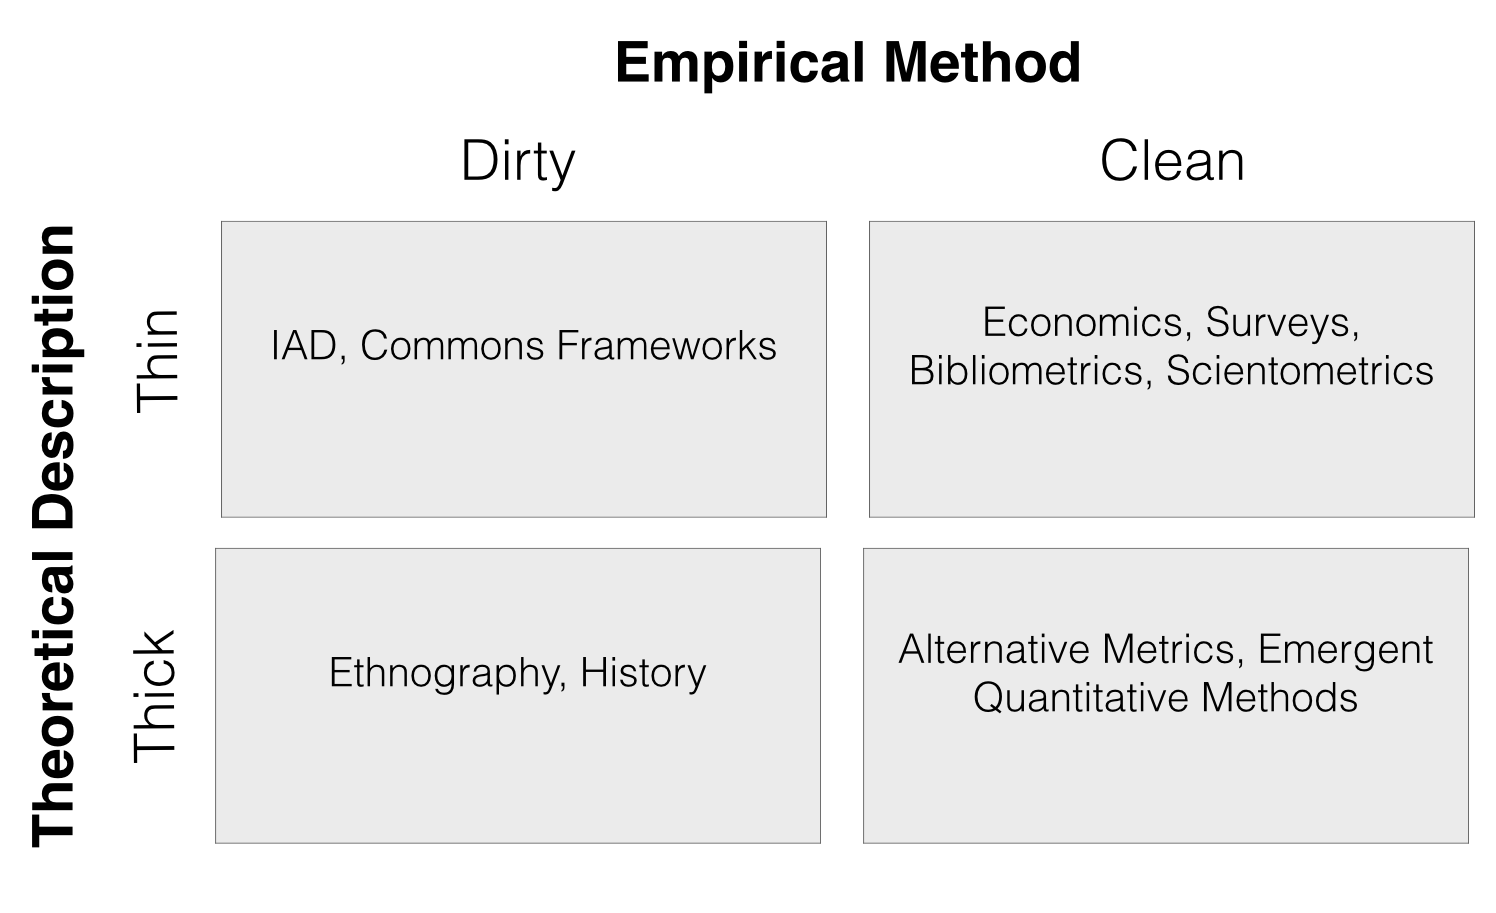
\includegraphics[width=\textwidth]{MethodsMatrix}
\caption{Matrix of Social Science Research \citep[adapted from][]{boettke2000review}}
\label{fig:my_label}
\end{figure}

The choice between different approaches to empirical research presents a
trade-off between``dirty'' or ``clean'' methods \citep{boettke2000review}. Clean empirical methods are characterized by narrowly scoped research questions, ordered and systematic data collection, and depend upon well
established thresholds of significance for the acceptance or rejection
of a research result. Dirty empirical research methods are, inversely, characterized by broad
research questions, opportunistic and informal data collection, and the
use of subjective judgment about the relevance of a research finding.\\

The other dimension of this matrix presents a trade-off between theories
used to analyze a research finding, and can be characterized as
producing either a ``thin'' or ``thick'' set of descriptions.\\

\parindent Thin theoretical descriptions often take the form of a framework that
can make the content of an explanation easily accessible to the reader.
Thin descriptions might use a narrowly defined theory to explain
research findings, or a set of ``most likely'' explanations applied to
selected research results. Thin theoretical descriptions often take the form of a framework that
can make the content of an explanation easily accessible to the reader. Thick descriptions often include a set of emergent theories about the
situated context in which some thing obtains meaning, or value. Thin descriptions lack depth in explaining the broader context of a
phenomena being studied, and are often unconcerned with the ``how and
why,'' and thick descriptions offer rich, but dense and non-linear narratives that
are open to many interpretations. 

\subsection*{Thick \& Dirty; Thin \& Clean}

At the intersection of these two dimensions -- dirty and clean, and
thick and thin- is where we can locate most social science research
projects.\\

To return to research projects described chapter two, Vertesi and
Dourish's study of ``data economies'' is an empirically dirty and
descriptively thick study of value. The authors present in rich detail
the different strategies and motivations for sharing data among two
research teams working at NASA's Jet Propulsion Laboratory (2011). The
results of this work take the form of broad ``implications'' for the
design of a future data management system.\\

Bollen, Fox and Singhal's conducted a study of the benefits of
supercomputer access to TeraGrid researchers is an empirically clean and
descriptively thin research project, answering questions like, ``Do
mostly high-impact scientists benefit from the TeraGrid?'' or ``Are some
scientific domains more strongly represented than others in
TeraGrid-supported work?'' \citeyearpar{bollen2011and}. The authors use highly normalized and
openly accessible citation data, and the findings are validated by
established statistical tests. While these results offer easily
digestible ``proof'' that the scientist's using the TeraGrid infrastructure have produced
papers with high citation rates, the author's thin
description of this phenomenon offers few details about how, or why the
TeraGrid publications have had an impact on the geoscience research
community. As they state, ``TeraGrid usage is indeed
significantly correlated with the scientific impact of its users, but
the causal direction of this relation remains unclear'' \citep[p. 11]{bollen2011and}\\

\subsection*{Thick \& Clean; Thin \& Dirty}

While the two approaches described above are well established modes of inquiry for social science research,  research projects that populate the opposite cells of this matrix are more rare. Some descriptively thick and empirically clean research can be
characterized as a ``kitchen sink'' approach where every possible
statistical test is thrown at a dataset to see what might emerge from
the results \citep{Boettke2000.  With increased access to data and open-source ``plug and play'' software tools the descriptively thick and empirically clean research approach
is becoming more common. Topic modeling projects in the digital
humanities \citep{rosen2010learning}, social network analysis and data mining in computational social
science \citep{keegan2010dark}, and
the visualization of sentiment analysis in studies of social media use \citep{hochman2012visualizing} are all salient examples of research that is
descriptively thick and empirically clean.\\

In the opposite cell, descriptively thin and empirically dirty research
would ask broad research questions about diverse subjects and use
research methods such as participant interviews or ethnographic methods which are impossible to reproduce. These types of research projects would then generate highly structured descriptions by using the conventions of a previously developed framework -- producing thin
descriptions of a phenomenon by abstracting from the messiness of an
empirically dirty method. As an example, the Institutional Analysis and
Development (IAD) framework achieves this by asking broad research
questions, like ``What motivates fishermen to cooperate with one another
in sustaining a fishery'' \citep{hutchings1994can} and uses
field-based research methods such as participant observation,
interviews, and surveys to gather behavioral data about individual
stakeholders. Researchers using the IAD are then guided by a
well-established framework that categorizes and organizes the data for analysis. There may seem to be a high investment for a small payoff in the descriptively thin and empirically dirty approach, but this mode of inquiry also presents a way to overcome the n = 1 shallowness of a case study.
Results fitting into a structured form of analysis makes it possible for
the n= 1 formula to actually become an n = X + 1 where X represents an
archive of comparable studies.\\

\subsubsection*{Research in This Dissertation}

The studies presented in chapter one both used empirically clean
research methods, but differed in the presentation and interpretation
of their respective research results. In the Data Usage Index we used data which were publicly available and a set of adapted, but well accepted measures of
impact \citep{weber2013product}. Consequently the description of our results were thin in
reporting quantitative scores across a variety of data products with
little ability to interpret their broader contextual meaning. The genealogical study of ICOADS also used publicly available data and well accepted 
techniques from evolutionary biology for our analysis \citep{thomer2014phylo}. In that the application of those techniques were novel our descriptions of those results were broad, highly subjective and our description was undoutedly thick.\\

The case study described below will be a quintessentially thick and
dirty research project, with all of the benefits and drawbacks of an n=1
study as described above. My argument from chapter one is that by over
relying on this mode of inquiry in studying eScience collaboration and
resource sharing, social science is failing to adequately inform federal
science and technology policy \citep{jackson2013cscw}.
The contribution this dissertation will make is creating a framework that can turn the n = 1 shallowness of the case study approach to developing theory, into the n = X + 1 power of an analytical framework. This will be done by first analyzing relevant features from four existing frameworks, and fitting the findings of the case study data to these features using an iterative process. This work has initially built off of existing efforts to extend the IAD framework to cultural commons settings \citep[e.g.]{adison2010constructing}.\\

In the following sections I describe the design and protocol for completing a case study of ICOADS. This case study will shed light on the complexity of this particular project, and demonstrate the need to develop a framework for studying similar cases. I then describe a parallel process for using the data from the case study to develop a framework which can help identify important, emergent properties in these settings. Again, the goal of this work is to develop a diagnostic tool which can be used to conduct multi-method social science work in collective action settings.\\

\section{Case Study}

The case study approach to social science research includes ``the logic
of design, data collection techniques, and specific approaches to data
analysis," it is not so much a method as it is a comprehensive research
strategy \citep[p. 14]{yin2003case}. The marked features of a case study are that
it:\\

\begin{itemize}
\itemsep1pt\parskip0pt\parsep0pt
\item
  Investigates a contemporary phenomenon within its real-life context
\item
  Is appropriate when the boundaries between phenomenon and context are
  not clearly evident
\item
  Copes with the technically distinctive situation in which there will
  be many more variables of interest than data points,
\item
  Relies on multiple sources of evidence, with data needing to converge
  in a triangulating fashion. and
\item
  Benefits from the prior development of theoretical propositions to
  guide data collection and analysis \citep[Quoted from][]{yin2014case}.
\end{itemize}

The collective action problems and dilemmas addressed in this proposal
draw upon theories of human organization that attempt to explain how ``a
group of principals can organize themselves voluntarily to retain the
residuals of their own efforts'' \citeyearpar[p. 25]{ostrom1990governing}, and more
specifically how it is that individuals and institutions with
overlapping research agendas are able to resolve these conflicts, and
coordinate their actions to successfully cooperate over long periods of
time.\\

In social science research that takes things like organizations,
institutions or systems as a unit of analysis, the case study approach
can be used either to test, extend, or further develop existing theories \citep{stake1995art}. A case study aproach can also act as the operational strategy for putting an existing methodological framework into action. In the latter sense, a case study sets out a design for collecting data based on specific questions to be answered by a specific case. The case study will identify variables in a framework to decide what is to be studied, how a method will be used to find out what is asked of or about the specific context of these variables, and how the gathered data will be linked to the categories of
the framework for analysis.\\

A case study, like a framework, can mean very different things to very
different fields engaged in social science research. Yin identifies three types of case studies:\\

\begin{enumerate}
\def\labelenumi{\arabic{enumi}.}
\itemsep1pt\parskip0pt\parsep0pt
\item
  Exploratory - often experimental, and aimed at developing or refining
  a general thesis. The exploratory case study is valuable for
  investigations which are emergent, or where little research is
  available to support existing theories.\\
\item
  Descriptive - often uncovers phenomena that are not well understood,
  or oversimplified. The descriptive case study is important in
  clarifying how a well accepted theory, such as social deviance \citep{becker1967whose} applies to a
  new environment (i.e.~social networking sites).
\item
  Explanatory - seeks to make meaning of an event, policy, or period
  -asking why it occurred, how it was resolved or what outcomes mean for
  contemporary (or future) settings \citeyearpar{yin2003case}
\end{enumerate}

A fourth type of case study that is related to both the descriptive and exploratory is the
critical or paradigmatic case study. The critical case study identifies a single case that
is exemplary in some way, such as a medical oddity that is rare, a
revolutionary social movement, or as was explored by Kuhn evidence of
some larger pattern that could only be supported by the in-depth study of an
exemplary case \citep{kuhn1962structur, flyvbjerg2006five}. I earlier argued that we
can see ICOADS as a kind of sociotechnical
system that will become more prevalent in the coming years. This is a
result of shrinking federal support for basic science research and
consequently the need to pool shared resources, but also more
practically as the type of institutional arrangement needed to tackle
systems-based grand challenge science problems. My case study of ICOADS is most comparable to the critical case study, but takes on many
characteristics of the explanatory model.\\

\subsection*{Research Design}

The five components to case study research design require the following:

\begin{enumerate}
\def\labelenumi{\arabic{enumi}.}
\itemsep1pt\parskip0pt\parsep0pt
\item
  A study's questions
\item
  Propositions
\item
  Unit(s) of analysis
\item
  Logic linking the data to the propositions
\item
  Criteria for interpreting the findings (Yin, 2003). 
\end{enumerate}

In the following sections I describe my design of a critical case study
for ICOADS using these five components.

\subsubsection*{Research questions}

The research questions this case study will address are:\\
\textbf{RQ1} : How does ICOADS, as an institution for collective action,
overcome transaction costs in organizing its production of new
knowledge? If peer production is indeed the model by which this is
achieved:

\begin{itemize}
\item[]
  \textbf{RQ 1.1} How, and/or in what ways does it differ form other forms of
  peer production?
\item[]
  \textbf{RQ 1.2} How does ICOADS sustain these successful cooperative
  arrangements
\item[]
  \textbf{RQ 1.3} What are the activities of its community members necessary to
  achieve this sustained success, and how can those actions be
  recognized, either formally or informally, over the duration of the
  project's existence?
\end{itemize}

\textbf{RQ2.} How has ICOADS, as a project with particular governance
arrangements, evolved in response to external pressures from funding
agencies, the politicization of climate related research, and rapid
technological change?\\

Both of these questions are answered in the context of events occurring
after the 2012 defunding of NOAA's Earth Systems Research Laboratory,
but the examination of how these events are similar to or different from
historical ones are necessarily important to interpreting the findings
of this work. That is to say, while case studies are typically concerned
with ``contemporary phenomena'' they are of limited value unless they are able to answer
these questions in a broader historical context.
Diane Vaunghn's work on NASA's \emph{Challenger} and \emph{Columbia}
accidents is an exemplar for this type of case study \citeyear{vaughan1996challenger, vaughan1999role}. Her analysis is
grounded in contemporary events, but through archival work she necessarily
reflects on the organizational and institutional factors that led to the
present. Vaughn describes this process as historical ethnography \citep{vaughan2006nasa}.\\

\subsubsection*{Propositions}

Propositions stated in a case study are usually some combination of a
priori and a posteriori knowledge about the unit of analysis, the
context or setting in which a subject will be studied, and the research questions that
will be asked of those settings. My work with the ICOADS community in
developing the DUI and Genealogy of ICOADS data led to generating
research questions about the evolution of cooperation, and the
sustainability of collective action in this environment. In chapter two
I defined and gave examples of research applicable to ICOADS,
and this in turn helped me generate the following set of propositions:\\

\begin{itemize}
\itemsep1pt\parskip0pt\parsep0pt
\item
  ICOADS is a peer produced resource. As such, it has qualities that are
  similar to commons-based peer production systems that follow a
  heavyweight model.
\item
  However, ICOADS contributors and users largely consist of experts, and it
  therefore diverges in important ways from traditional 
  peer production models that loosely coordinate non-experts.
\item
  Changes in any one of the technical, social, political, or economic
  aspects of ICOADS partners will impact broader peer production arrangements, and the project's overall
  ability to solve collective action problems.
\item
  These changes will impact participants differently (benefiting some,
  harming others).
\item
  Solutions to collective action problems adopted by ICOADS will be
  similar to those found in Ostrom's study of common-pool resources.
\item
  In particular, the concept of polycentricity will play an important
  role in how institutional arrangements evolve.
\item
  However, effective solutions for collective action will look different than common-pool
  resources like Spanish Huertas (Ostrom, 1990), and Open Source
  Software projects (Schweick and English, 2012) as a result of ICOADS
  being made up of quasi-public-goods.
\end{itemize}

\subsubsection*{Unit of Analysis}

In short, a unit of analysis is the subject of a case study \citep{Long2004}. A related but distinct concept is the unit of observation, which
is often a manifestation of the subject being analyzed. To return to an
example used earlier in this chapter, Vertesi and Dourish's study at
NASA's JPL used ``data sharing between mission teams'' as a unit of
analysis, and individual teams and team members as units of observation. Case study research also draws a distinction between holistic (single
unit of analysis) and embedded (multiple units of analysis) \citep[p. 40]{yin2003case}\\

The case study design for this dissertation is a single-case (ICOADS)
with a single unit of analysis (cooperation in solving collective action
problems between project partners) and multiple units of observation, including digital resources
(ICOADS software and data) and curators, users and stakeholders of the
ICOADS project.\\
\subsubsection*{Data collection method}

The mode of inquiry I've used during the two years of engagement with
the ICOADS community has been influenced by ethnomethodology as found in
cultural anthropology \citep[e.g.][]{garfinkel1967studies} and science and technology
studies \citep[e.g.][]{lynch1997ethnomethodology}, but it is most directly informed by Harry
Collins' work on ``participant comprehension'' \citeyearpar{collins1987expert}. In studying the
material culture of gravitational wave physics, Collins described this
method as ``an interpretation of participant observation under which the
field-worker tries to acquire as high a degree of native competence as
possible and interaction is maximized without worrying about disturbing
the field site'' \citeyearpar[p. 297]{collins1998meaning}. Collins' motivation for developing this method is
in pursuit of an ``interactional expertise'', or a third kind of
knowledge that sits between formal / propositional knowledge and
informal / tacit knowledge \citeyearpar[p. 125-7]{collins2004interactional}.\\

Collins' argument is that
during his time studying gravitational wave physics he was able to
achieve an expertise which was something different than the kind that
comes with formally studying and being a part of a discipline as a
practitioner. Through linguistic socialization, traditional
ethnographic observation, and extended field work Collins could read,
participate in discussions, and defend his arguments about physics
without having the ability to actually do the physics himself.
Similarly, Anthony Giddens has described a similar mode of work, saying
``I have accepted that it is right to say that the condition of
generating descriptions of social activity is being able in principle to
participate in it. It involves `mutual knowledge,' shared by observer
and participants whose action constitutes and reconstitutes the social
world'' \citep[p. 15]{giddens1982profiles}.\\

My time working with and
studying ICOADS has allowed me to develop something like a ``mutual
knowledge'' or an ``interactional expertise'' in that I understand the
limitations and uses of ICOADS software and data in ways that allow me
to converse with its community, to read, comprehend and participate in
discussions of its literature, and most importantly to argue - a crucial
point of linguistic socialization \citep{collins1998meaning}- with one or more of
the conflicting theories in the field of marine climatology. I've even
given an invited talk at a biennial marine climatology meeting, which is
the major professional conference for the ICOADS community \citep{weber2014coop}.\\ 

My use of``participant comprehension'' expands on
Collins method by conceiving of participants more broadly. That is to
say, my ``field-site'' is not simply a series of laboratories, offices
or even people. I locate my phenomena of interest (sustainability of
collective action) mostly in digital environments: the logs of data
repositories, the encoding standards of ICOADS, and the many engineered
institutions and artifacts that make up this cooperative. Like Collins,
my interaction is ``maximized'' by informally interviewing, talking
with, and observing people who produce and use ICOADS; but, I also
interact with and investigate ICOADS by using it's various forms,
visualizations and software. I generate questions to investigate not only through the ``linguistic socialization'' that Collins describes \citep{collins1998meaning}, but also through a kind of ``material socialization'' by both using ICOADS myself, and studying it in different formal and informal environments of
use.\\

The questions, and categories that have driven this work are the outline of a
a framework, borrowed and adapted from multiple existing frameworks that
I review in the second half of this chapter. Further details on the
methods and data collection techniques can be found in Appendix A.\\

\subsubsection*{Linking Data to Propositions and Interpreting Findings}

Without formal methods for determining the truth value of a proposition, or the statistical significance
of a finding case study research depends on inductive data analysis techniques such as triangulation \citep[p. 133]{denzin2008strategies}, pattern matching, and a ``replication logic''
\citep{eisenhardt2007theory}. Undoubtedly the major critique of case study
research is that this step is performed too casually resulting in
underdeveloped theory or thin explanations of a phenomena \citep{flyvbjerg2006five}.
Case study research can guard against this critique by using various
forms of data validation, including:\\

\begin{itemize}
\item
  \textbf{Construct Validity}: Requires the careful selection of a case, a unit
  of analysis, using multiple sources of evidence, and selecting key
  informants that are willing to read the work being produced
\item
  \textbf{Internal Validity}: Is largely applicable to causal explanations, and
  requires intensive pattern matching, repeated findings across cases,
  building a logic model, and addressing rival explanations in answering
  a set of propositions.
\item
  \textbf{External Validity}: Concerns the generalizability of the findings, and the extent to which they are representative of a phenomenon in
  different contexts. In single cases, external validity is addressed
  through the use of theory, and comparing or contrasting the support of
  that theory with the explanations produced from a case study.
\item
  \textbf{Reliability}: Deals with the repeatability (not replication) of a case
  study. This is addressed thorough documentation, and a well
  developed protocol \citep{yin2003case}.
\end{itemize}

At this stage of my research, I can only address issues of construct
validity and reliability. For the former I have relied on a key
informant at NCAR who has collaborated with me on both studies presented
in chapter one, introduced me to members of the ICOADS community for
interviewing, and provided me with archival material for historical
portions of this work. He has agreed to read and provide feedback on
future iterations of this dissertation. For reliability, I have modified a protocol developed and tested in previous work \citep{weber2014extending}.
This protocol outlines how data are to be recorded, coded, stored and managed.
Details of the protocol can be found in Appendix A.\\

\subsubsection*{Progress on Case Study to Date}

As of August 01, 2014 I have completed a total of 15 months in residency at NCAR,
working with software engineers and the director of the RDA. This time has included data gathering as both
an observer and a participant in ICOADS curation. I have completed 7
informal interviews - including developers (n=4) scientists (n=2) and an employee of the Joint Technical Commission for Oceanography and Marine Meteorology (JCOMM) (n=1).\\

I have participated in four conferences related to ICOADS research and
development, as well as a workshop for the design and planning of a
ICOADS Value-added Database (IVAD). During these sessions I recorded
field notes following methods from Emerson, Fretz and Shaw \citeyearpar{emerson2011writing} on
ethnographic fieldwork. These data are further condensed to memos that
will be used to test portions of the framework described in the next
section.\\

There are a number of limitations of the data that I've collected for the case study thus far. In particular, I need to gain a better understanding of ICOADS from end-users (not people directly funded to work on or develop ICOADS). To date my interactions with the ICOADS community outside of NCAR has been opportunistic and based on who has attended major
conferences / workshops or who is connected to ICOADS through my key informant at NCAR. Over the next four months I plan to continue collecting data by participating in IVAD's planning (teleconference calls), as well as
interviewing a broader range of ICOADS stakeholders. I will
prioritize individuals who are not directly related to NCAR or NOAA, with a target of conducting five additional interviews.\\

\subsection*{Outcomes and Contribution of Case Study}
A chapter of this dissertation will be devoted to findings from this case study. I will use the propositions that I've stated to frame this work, showing how or why they were supported by my interactions with the ICOADS community. The analysis of events occurring after the 2012 defunding event will be the major focus of this work. In abstracting from the propositions to the research questions I will directly address how ICOADS as an institution for collective action overcame these issues, and the ways that this related to how peer-production systems evolve in the face of conflict. These events will be historically contextualized using the reflection of my participants and archival material relating to ICOADS, as well as literature that I reviewed in chapter two.\\ 

Data gathered during the case study will also be used to develop a framework, as described below. 

\section{Framework}

In chapter one I argued that if science and
technology policy is to move beyond simple panaceas for solving the
complex interrelated problems of sustaining sociotechnical systems then
an analytical framework is needed to address interactions
between different types of variables (resources, users, technologies)
and different levels of institutional interaction (disciplinary,
organizational, funding agency, etc.)\\

My third research question is about how
existing frameworks can be adapted for these purposes.\\

\begin{quote}
\textbf{RQ3}: How can analytical frameworks successful for studying
collective action problems in other domains be modified for
sociotechnical settings where issues of sustainability, cooperation and
shared resource management are diverse and shifting over time?
\end{quote}

In this section I will define the differences between frameworks, theories and
models in social science research related to institutions and
organizations. I will then describe the process I've used thus far to analyze existing frameworks, and a preliminary draft of a new framework. I'll conclude with the future steps necessary to complete the framework and a schedule for completion.\\

\subsection*{Frameworks, Theories, and Models}

A \textbf{Framework} can mean different things to different fields engaged in
social science work. For the sake of this dissertation, ``Frameworks
provide a meta-theoretical language that can be used to compare
theories. They attempt to identify the universal elements that any
theory relevant to the same kind of phenomena needs to include''
\citep[p. 8]{ostrom2011background}. A framework provides a set of relevant concepts and variables that need to be recorded and explained in the study of a given phenomenon. In analyzing the data that a framework generates either new theories emerge, or existing theories are applied in an attempt to make sense of a given situation.\\

"\textbf{Theories} posit general causal relationships among some subset of these
variables or categories of factors, designating some types of factors as
especially important and others as less critical for explanatory
purposes. Theories are used to focus in on one more parts of a framework
in order to 'diagnose a phenomenon, explain its processes, or predict
its outcomes\ldots{}'' \citep[p. 28-9]{ostrom1990governing}' \citep[p. 170]{mcginnis2011introduction}. I take theories to
have different kinds of powers -- descriptive; rhetorical; inferential;
as well as having different forms of application \citep{halverson2002activity}. Each of these powers
are emphasized or demoted based on the systematic gathering of data that
a framework enables. Some frameworks are good at testing and comparing theories that are inferential, and others are good at generating useful descriptions.\\

\textbf{Models} specify the ``specific functional relationships among particular
variables or indicators that are hypothesized to operate in some
well-defined set of conditions''\citep{mcginnis2011introduction}. In a sense, models put theories to work.  Models are not exact
simulations of reality, but always a simplification of some larger
complex system. When used in a sociotechnical setting models are useful for understanding or demonstrating the consequences of policy decisions (Easterbrook, 2014). In some cases a simplification is
helpful to understand basic causal relationships, and in other situations models can prove valuable for predicting or modeling a given outcome.\\

This dissertation will develop a \textbf{framework} for analyzing peer production arrangements, their sustainability, and their processes for solving collective action problems that arise from the pooling and sharing of research objects over time. The framework will provide a consistent vocabulary for important variables and their roles in a peer production process (resources, users, technologies) as well as different levels of institutional interactions (disciplinary, organizational, funding agency, etc.). I describe this process in detail in the following section.\\

\section{Stepwise Development of Framework} 

The development of a framework to support the analysis of sustainability will be done using a stepwise process that adds concepts, variables or levels of interaction as necessary, and decreases the number of overlaps where possible. My work on this development process includes the following (non-sequential) steps:\\

\begin{enumerate}
\item
Analyze a set of pre-existing frameworks for features relevant to sustainability, longitudinal analysis, sociotechnical systems, peer production and common property regimes. The initial analysis of these frameworks can be found in Appendix B.   
\item 
Incorporate relevant features from this analysis into a preliminary set of questions to be addressed in gathering case study data (below).
\item 
Identify relevant concepts from systems theory literature, which provides a domain ontology to capture concepts like stocks and flows, balancing and feedback loops, and emergent behaviors in dealing with complexity in built or engineered environments \citep[such as ICOADS][]{weinberg1975introduction, easterbrook2014computational}.
\item 
Develop new categories not found in existing frameworks. 
\item 
Identify the different levels of analysis necessary for a sustainability framework (policy relevant levels, operational levels, etc)\footnote{Identifying different "levels" of systems analysis is sometimes referred to as a process of "boundary critique" in complexity theory \citep[e.g.][]{midgley1998theory} }. 
\end{enumerate}


As a brief demonstration of this process, I can explain a portion of my preliminary work as follows:\\
\begin{itemize} 
\item  I began by analyzing four frameworks: the Institutional
Analysis and Development framework from Ostrom and McGinnis; the Constructed
Cultural Commons framework by Madisson, Frischmann and Strandburg; the
Sociotechnical Interaction Network by Kling, McKim and King; and the
Multi-dimensional In-depth Longitudinal Case Study framework by
Schneiderman and Plaisant.\\
\item 
Using the highest level categories from the IAD \citep{mcginnis2011introduction} I outlined what each category was trying to achieve in studying a socio-ecological system. 
\item
I then identified what was similar and was different about ICOADS as a sociotechnical system (i.e. ICOADS is an engineered system, not a naturally occurring huerta) 
\item 
Most studies of a socio-ecological system using the IAD had the following features.
\begin{enumerate}
\item
The boundaries between resources were clear 
\item
The resource systems studied were relatively small, well bounded, and easy to observe. 
\item
Overcoming collective action problems was immediately important to some aspect of the community's existence (water, food, shelter, etc.)
\item
The institutions for collective action were relatively long-enduring and had evolved over time, and 
\item
The ability to spend time in the field observing, or interviewing was available and relatively unobtrusive \citep[Quoted from][]{ostrom2011background}. 
\end{enumerate}

Each of these assumptions is complicated, if not completely opposite for peer produced commons of digital material: 
\begin{enumerate}
\item 
Boundaries are unclear 
\item
While access to resources are important to efficient research, alternative means of access do exist (this became clear during the federal government shutdown of 2013 when many NOAA scientists started to access ICOADS data from NCAR) 
\item
Resource systems are large, distributed across many different platforms.
\item
Institutions are rapidly evolving and often short-lived or unrecognizable from one project to the next (i.e. a code base exchanged between projects).
\item
Due to the size and nature of collaborations (virtual), traditional observation techniques are not possible.   
\end{enumerate}
\end{itemize}
\\

To account for these differences I changed the first level of analysis of the IAD from 'Exogeneous Biophysical Characteristics' to 'Sociotechnical Contexts.' This level of analysis for my framework includes questions about the type of good produced (public, private, common-pool, etc), and questions about the significant properties of the good. These are meant to deal with problems of boundaries that exist between different types of goods. Below is the first draft of the framework that I have developed. Following this draft is a section that describes the process for completing the framework development.

\section*{Preliminary Design of Framework}

\emph{Current categories include sociotechnical contexts, actions and actors, and outcomes and evaluations. I describe each section in detail below.} 

\section*{Sociotechnical Contexts}
\subsection*{Resource Characteristic}

\begin{list}{\quad}{}
\item[]
\textbf{Type of Good}: Is the good managed as a private, public, or club
good? To what degree is there rivalry for the resource? Are there
barriers to access and use? How are barriers enforced?\\

\textbf{Significant Properties}: 
(Traditional software significant property categories are content, context, rendering, structure, and behavior) What does the resource consist of? What
platforms or systems is it used on? What are the standards to describe, encode, or archive this good? What are its known dependencies, and howhave these evolved over time? Does the resource exist in many locations?
Many versions? What are the salient differences among these versions?\\
\end{list}


\subsection*{Attributes of Community}

\textbf{Reciprocity:} Do members of this community share the common
expectation that others will tend to reciprocate their own acts of
cooperation? How, and to what extent? (McGinnis, 2011) \\

\textbf{Trust:} Do members of community exhibit reciprocity ? Is this reflect, for instance, in citation analysis or other formal methods of acknowledgement? How do members describe goods in terms of quality, reliability, care, etc.?\\


\textbf{Common Understanding (or
shared understanding):} What values and conceptual frameworks do the
members of this community share, and specifically do most of them share
at least some core values or goals as a member of that
community? How are the commonalities expressed? Is there documentation of expectations? Memorandums of understanding? Is there a license that is attached to goods stating these expectations about fair use. etc.?\\

\textbf{Social Capital:}, can be studied by analyzing the resources that an individual can access, and their understanding or belief that they can obtain goods that are not within their immediate network? ( Can be addressed through forums, question and answer sites, listservs, etc.). Can also be studied with a survey that asks participants to report knowledge of certain resources and ability to access or obtain others \citep[i.e.][]{appel2014testing} \\

\textbf{CulturalRepertoire:} What are the set of strategies, norms, rules,
organizational templates, and other remembered or imagined practices
that are readily available to the members of that community for their
use in processes of deliberation and implementation? (McGinnis, 2011)\\

\subsection*{Rules in Use:}\\
\textbf{Formal Rules:} To what extent are rules codified in a formal
document, mission statement or memorandum of understanding? Do community
members refer to these documents? Where are these documents stored, made
available to new members, and referred to when conflicts arise?\\

\textbf{Strategies for Deviance:} What are the norms or rules being
used on a regular basis by participants that diverge from or mirror the
formal rules? \\

\section*{Actions + Actors}
\subsection*{Action Situation}
This is essentially the unit of analysis for applying a framework. The questions
to be answered then are about how actors (broadly construed) observe
information, select actions, engage in patterns of interaction, and
realize outcomes from their interactions.\\

\subsection*{Actors}
The term actor here is broadly
construed as both human agents and software agents. The reasons should
not be confused with anthropomorphism, but instead how a community
conceives of and attributes action with respect to the sustainability of
a resource. The inspiration for this treatment is Callon's study of
networks of translation between fisherman, scientists, consumers and
scallops where he noted that in his unit of analysis (the network) a
difference between intentional and unintintentional action did not
matter, ``The only thing that counts is the definition of their
{[}scallops{]} conduct by the various actors identified. The scallops
are deemed to attach themselves {[}to certain types of breeding
grounds{]} just as fishermen are deemed to follow their short term
economic interests. They therefore act.'' \citep[p. 25, bracketed
content was added by me for sake of clarification]{callon1986some}. In ICOADS case, data
processing algorithms, floating buoys, satellites, models of physical
systems, and software act in the same way that scientists, curators and
funding agents do. The questions to answer about actors then are not
whether or not they act intentionally, but instead who or what has
agency?\\ 

\subsection*{Outcomes and Evaluation}

\subsubsection*{Outcomes}
The outcomes of action scenarios can take many different forms. For the sake of this
dissertation, which is concerned with the sustainability of collective
action, I evaluate outcomes based on the evaluative criteria discussed
below. These will need to be adjusted in many different settings (McGinnis, 2011)\\

\subsubsection*{Evaluation}

Six forms of an outcome are identified as the efficiency, equity, legitimacy, and fiscal
equivalence of an action situation (McGinnis, 2011).\\ 

\textbf{Efficiency} in use of
resources, especially capture of economies of scale.\\

\textbf{Equity} in
distributional outcomes and processes.\\

\textbf{Legitimacy} as seen by
participants in decision processes (participation tends to increase
legitimacy)\\

\textbf{Accountability} especially to direct users of
resource.\\

\textbf{Fiscal equivalence:} the extent to which the
beneficiaries of a public good or service are expected to contribute
towards its production.\\

\textbf{Consistency} with the moral values
prevalent in that community.\\

\section{Completion of Framework}
The steps taken to finish the framework will be similar to that of other inductive approaches that depend on an itterative process of making sense of data, fitting explanations to abstract categories, and reaching a point of saturation in explaining the phenomena under study \citep{suddaby2006editors}. In the completed dissertation each category will be defined, and an example from ICOADS will be used to demonstrate their significance. Where possible, I will relate this to relevant literature or my own previously published work in order to demonstrate the ability of the framework to accommodate different eScience contexts. 

\newpage
\section{Limitations of Proposed Study}

There are a number of limitations to the study I am proposing. 
In the case study, I have had a limited set of interactions with a large and
diverse international project. I have attempted to guard against this limitation by attending international conferences related to ICOADS, and in interacting with visiting scholars at NCAR.\\ 

Although I've developed a high competency in this field, I nonetheless have an incomplete understanding of marine
climatology and climate science more generally.\\

During my time interacting with participants, I did not record my interviews. This
decision was made to be least disruptive and most natural to the community I was
collaborating with, and my own reluctance to ask a group of individuals whose
work is highly politicized to be tape-recorded.\\

All single-case study work suffers from a lack of generalizablity. The protocol that I have developed and the validity measures
described above will be important for assuring a rigorous and empirical
study is conducted, but the results from this work will still be limited
in their scope of the sustainability and collective action problems facing eScience.\\ 

An important aspect that I will have to address in the completed dissertation is how and to what extent this framework is adaptable to a broader research community. It may be that portions are very succesful and others are not (i.e. What can this framework achieve with respect to different levels of intraction that something like Weinburg's 'principles of complimentarity' cannot? \citeyearpar{weinberg1975introduction}. \\

\newpage
\section{Timeline for Completion}
\begin{table}[h]
\resizebox{\textwidth}{!}{%
\begin{tabular}{lllllllll}
 &  & \multicolumn{7}{c}{\textbf{Aug. 2014 - Feb. 2015}} \\ \cline{3-9} 
 & \multicolumn{1}{l|}{} & \multicolumn{1}{l|}{Aug} & \multicolumn{1}{l|}{Sept} & \multicolumn{1}{l|}{Oct} & \multicolumn{1}{l|}{Nov} & \multicolumn{1}{l|}{Dec} & \multicolumn{1}{l|}{Jan} & \multicolumn{1}{l|}{Feb} \\ \hline
\multicolumn{1}{|l|}{\textbf{Case Study}} & \multicolumn{1}{l|}{Complete Data Collection} & \multicolumn{1}{l|}{\cellcolor[HTML]{C0C0C0}} & \multicolumn{1}{l|}{\cellcolor[HTML]{C0C0C0}} & \multicolumn{1}{l|}{\cellcolor[HTML]{C0C0C0}} & \multicolumn{1}{l|}{} & \multicolumn{1}{l|}{} & \multicolumn{1}{l|}{} & \multicolumn{1}{l|}{} \\ \hline
\multicolumn{1}{|l|}{\textbf{}} & \multicolumn{1}{l|}{Data Analysis} & \multicolumn{1}{l|}{} & \multicolumn{1}{l|}{\cellcolor[HTML]{C0C0C0}} & \multicolumn{1}{l|}{\cellcolor[HTML]{C0C0C0}} & \multicolumn{1}{l|}{\cellcolor[HTML]{C0C0C0}} & \multicolumn{1}{l|}{\cellcolor[HTML]{C0C0C0}} & \multicolumn{1}{l|}{} & \multicolumn{1}{l|}{} \\ \hline
\multicolumn{1}{|l|}{\textbf{}} & \multicolumn{1}{l|}{Written Narrative of Findings} & \multicolumn{1}{l|}{} & \multicolumn{1}{l|}{} & \multicolumn{1}{l|}{\cellcolor[HTML]{C0C0C0}} & \multicolumn{1}{l|}{\cellcolor[HTML]{C0C0C0}} & \multicolumn{1}{l|}{\cellcolor[HTML]{C0C0C0}} & \multicolumn{1}{l|}{} & \multicolumn{1}{l|}{} \\ \hline
\multicolumn{1}{|l|}{\textbf{Framework Development}} & \multicolumn{1}{l|}{Comparison of Frameworks} & \multicolumn{1}{l|}{\cellcolor[HTML]{C0C0C0}} & \multicolumn{1}{l|}{\cellcolor[HTML]{C0C0C0}} & \multicolumn{1}{l|}{} & \multicolumn{1}{l|}{} & \multicolumn{1}{l|}{} & \multicolumn{1}{l|}{} & \multicolumn{1}{l|}{} \\ \hline
\multicolumn{1}{|l|}{\textbf{}} & \multicolumn{1}{l|}{First Draft of Framework} & \multicolumn{1}{l|}{} & \multicolumn{1}{l|}{} & \multicolumn{1}{l|}{\cellcolor[HTML]{C0C0C0}} & \multicolumn{1}{l|}{\cellcolor[HTML]{C0C0C0}} & \multicolumn{1}{l|}{\cellcolor[HTML]{FFFFFF}} & \multicolumn{1}{l|}{} & \multicolumn{1}{l|}{} \\ \hline
\multicolumn{1}{|l|}{\textbf{}} & \multicolumn{1}{l|}{Final Version of Framework} & \multicolumn{1}{l|}{} & \multicolumn{1}{l|}{} & \multicolumn{1}{l|}{} & \multicolumn{1}{l|}{} & \multicolumn{1}{l|}{\cellcolor[HTML]{C0C0C0}} & \multicolumn{1}{l|}{} & \multicolumn{1}{l|}{} \\ \hline
\multicolumn{1}{|l|}{\textbf{Completed Dissertation}} & \multicolumn{1}{l|}{First Draft to Committee} & \multicolumn{1}{l|}{} & \multicolumn{1}{l|}{} & \multicolumn{1}{l|}{} & \multicolumn{1}{l|}{} & \multicolumn{1}{l|}{} & \multicolumn{1}{l|}{\cellcolor[HTML]{C0C0C0}} & \multicolumn{1}{l|}{} \\ \hline
\multicolumn{1}{|l|}{\textbf{}} & \multicolumn{1}{l|}{Final Draft} & \multicolumn{1}{l|}{} & \multicolumn{1}{l|}{} & \multicolumn{1}{l|}{} & \multicolumn{1}{l|}{} & \multicolumn{1}{l|}{} & \multicolumn{1}{l|}{} & \multicolumn{1}{l|}{\cellcolor[HTML]{C0C0C0}} \\ \hline
\multicolumn{1}{|l|}{} & \multicolumn{1}{l|}{Proposal Defense} & \multicolumn{1}{l|}{} & \multicolumn{1}{l|}{} & \multicolumn{1}{l|}{} & \multicolumn{1}{l|}{} & \multicolumn{1}{l|}{} & \multicolumn{1}{l|}{} & \multicolumn{1}{l|}{\cellcolor[HTML]{C0C0C0}} \\ \hline
\end{tabular}
}
\end{table}

%\include{intro}	% for INTRODUCTION in "intro.tex"
%\include{exper}
%\include{concl}


%%%%%%%%%%%%%%%%%%%%%%%%%%%%%%%%%%%%%%%%%%%%%%%%%%%%%%%%%%%%%%%%%%%%%%%%%%%%%%%
% APPENDIX
%
\appendix
\section{Appendix A}

08/12/2104 - this content will be added to subsequent drafts, deposited at:
http://bit.ly/1ropvH6


\section{Appendix B}

\textit{In this Appendix are an initial analysis of four frameworks: the Institutional
Analysis and Development framework from Elinor Ostrom; the Constructed
Cultural Commons framework by Madison, Frischmann and Strandburg, the
Sociotechnical Interaction Network by Kling, McKim and King, and the
Multi-dimensional In-depth Longitudinal Case Study framework by
Schneiderman and Plaisant.}
\\
\subsection*{The IAD}

In the late 1980's, the
Bloomington school began to develop a more formal framework for studying
the evolution and function of commons. The Institutional Analysis and
Development (IAD) framework was to guide the analysis of data collected
through many different empirical methods. Various versions of this
framework can be found in the work of Kiser and Ostrom \citeyearpar{kiser2000three}, Ostrom
\citeyearpar{ostrom1990governing}, Ostrom, Gardner, and Walker \citeyearoar{ostrom1994rules}, and McGinnis \citeyearpar{mcginnis2011introduction}. The settings for much of this work
were institutions that operated with a mix of governance structures, and
had a need for longevity or sustainability of a single shared resource.
Initially the IAD was designed as method-agnostic tool that could
``simplify the analytical task confronting anyone trying to understand
institutions in their full complexity.'' \citeyearpar{mcginnis2011introduction}.\\ 

Another goal of this unifying framework was to integrate the work of sociologists,
lawyers, politicians, economists, and political scientists in trying to
understand how ``institutions affect the incentives confronting
individuals and their resultant behavior'' \citep{ostrom2009understanding}. While the
original goal may have been to simplify the task of studying
institutions in diverse settings, the IAD has been used, adapted and
modified so many times that it often seems incomprehensible as a single
framework. Below, I sketch out the most basic features of the
framework.The IAD divides an investigation into three levels of analysis
for studying ``underlying factors'' of an intsituion's success or
failure -- (1) exogenous variables, (2) action arenas, and (3) outcomes
and evaluations.\\

\begin{enumerate}
\item 
1. Exogenous variables include biophysical attributes of
the shared resources, community attributes, and structural governance
policies (formal or informal).Exogenous variables are also considered
the ``input'' to a complex system.\\ 
\end{enumerate}

In his overview of the framework
Frischmann gives a simple example of this group, from the Maine Lobster
fishing grounds, "\ldots{}attributes might include the relevant
biological characteristics of lobsters, such as the rates at which they
age and reproduce; attributes of the community of fishermen, such as the
proximity in which they live to others, the existence of familial
relationships, and the skill sets needed for lobster fishing; and the
rules---explicit or informal---that govern fishing." \citep{frischmann2013two}. The most crucial aspect of this level is that while individual
attributes or variables are identifiable and observable, they need not
be considered fully decomposable \citep{ostrom2009understanding} -- meaning that the
salient features of a commons are often thought to be ``emergent
properties'' where the mutual constitution of people and objects (in the
case of ICOADS technologies) create phenomena which are indivisible. The
use of multiple research methods for the same institutional setting are
often justified on the grounds of needing to understand these emergent
properties \citep{ostrom2009understanding}.\\

\begin{enumerate}
\item
2. An Action Arena -- space where exogenous
variables and actors interact, cooperate, and conflicts emerge. This level
of the IAD places the stakeholders and the resources of the commons --
as inventoried in level 1 -- into a particular setting such as the
harvest of a shared common field. Using the understanding gained from
level one, the analyst observes this process and then identifies
tangible outcomes, objective results and the way that conflicts from the
past, or the present are voiced, contested, settled or deferred. This
analysis can take place over long periods of time, to give a
longitudinal account of action such as the restoration of an aquifer
\citep{ostrom2010moving} or a statistical analysis of these processes
through agent-based models or multi-modal network analysis \citep{axelrod1997advancing}.\\
\end{enumerate}
\begin{enumerate}
\item
3. Outcomes and Evaluation -- the results and feedback of action
situations In the final stage of the framework an institution can be
evaluated based on outcomes of the action arena; that is, how well an
institution did or did not solve a collective action problem. Criteria
for evaluation will vary by institutional setting, but usually includes
calculation of transaction costs, such as (1) information costs (2)
coordination costs; and, (3) strategic costs, or
sustainability of the shared resource in terms of (1) efficiency in
access and use (2) equity of distributed wealth or costs, (3)
accountability for resource management, or (4) adaptability of the
institution in light of these outcomes  \citep{imperial2005taking}.\\ 
\end{enumerate}

\begin{figure}
\centering
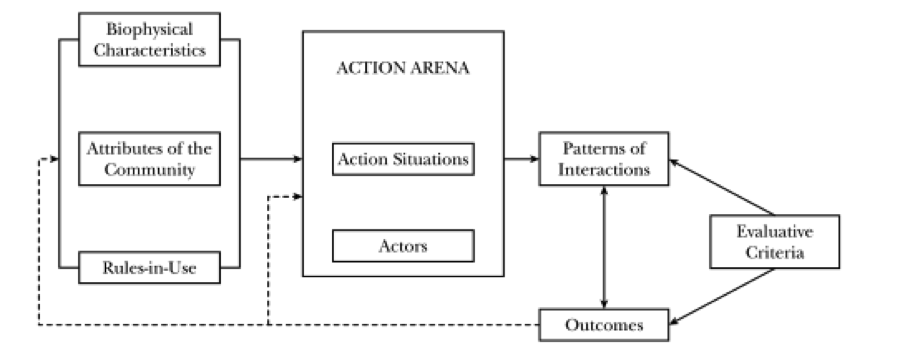
\includegraphics[width=\textwidth]{Ost}
\caption{The framework of the IAD (Ostrom, 2005, p.~15)}
\label{fig:my_label}
\end{figure}

For commons made up of natural resources, of the
type previously studied by institutional scholars: the boundaries were clear,  the resource systems studied were small and easy to observe, solving problems was of high salience to appropriators, institutions were long-enduring and had evolved over time, and (5)
extensive field observation was available \citep{ostrom2011background} Each of these
assumptions is complicated, if not completely opposite for peer produced
commons of digital material. Notably, boundaries are unclear, resource
systems (commons) are large, distributed and impossible to observe
qualitatively, and institutions are rapidly evolving- often existing for
short funding cycles that are of the 5-10 year range. While the IAD
provides a starting point, the dynamic nature of purposefully built
commons of digital objects requires much more innovation than a simple
re-tooling of terminology \citep{hess2007understanding}. In the next section I
review a proposal for the constructed cultural commons, which provides a
novel way to overcome some of these limitations.\\ 

\subsection*{Constructed Cultural Commons} 

In a broad ranging discussion of the purely functional
account of common property regimes, three lawyers - Maddisson,
Frischmann and Strandburg , propose a new framework for studying the
cooperative work of cultural institutions facing collective action
problems. In this account, ``constructed cultural commons,'' are defined
as, ``environments for developing and distributing cultural and
scientific knowledge through institutions that support pooling and
sharing of that knowledge in a managed way'' \citep[p. 659]{madison2010constructing}. Constructed cultural commons are, as MFS
explain, markedly different than the natural resource commons of Ostrom
et al's study, ``These environments are designed and managed with
limitations tailored to the character of those resources and the
communities involved rather than left to evolve via market transactions
grounded solely in traditional proprietary rights'' \citep[p. 659]{madison2010constructing}\\

Madison, Frischmann and Strandburg propose that in creating a unified
framework for studying the success and failures of diverse cultural
commons by aligning their ``social role and significance'' within nested
institutions. In particular, their framework is to be used for works of
pooled resources that are not subject to the same types of intellectual
property laws that govern private property or common-pool resources.
MFS's proposal does not suggest moving away from functionalism, but to
add to it through a form of `analytical narrative' \citep{bates2000analytical},
where ``In proper proportion, a humanistic and metaphorical inquiry into
information policy, on one hand, and a functional approach grounded in
social science models, on the other hand'' \citep[p. 673]{madison2010constructing}. Or in other
words, a unified framework that can account for new modes of knowledge
production, distribution and the purposeful construction of cultural
objects in physical and digital forms.\\

Their proposed framework achieves
this through three major innovations with the IAD: 1. It emphasizes among
distributed actors, and the constructed nature of the resources
themselves (purposefully built objects as opposed to natural
resources) 2. Where the IAD separates ``outcomes'' (level 2) and
``patterns of interactions'' (level 3) the constructed cultural commons
framework treats these as iterative, mutually constitutive processes. 3.
As a result of the more complex relationships between resources,
participants, and governance structures-- the ``relevant'' attributes of
each may not neatly divide into categories.\\ 

\begin{figure}
\centering
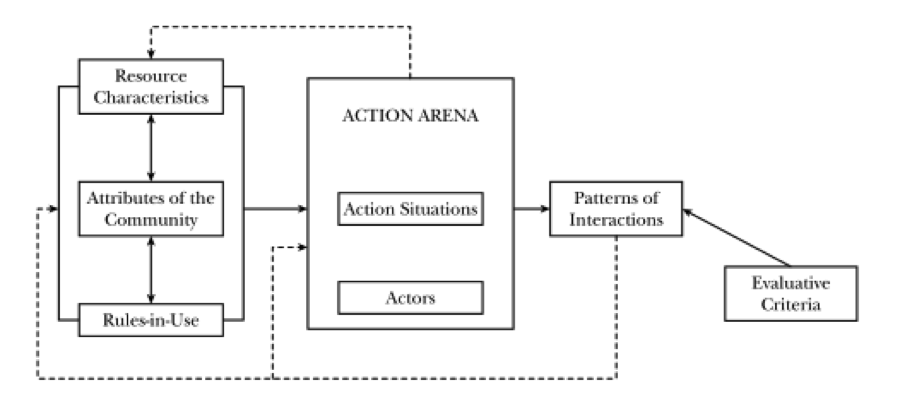
\includegraphics[width=\textwidth]{Mad}
\caption{Madison, Frischman and Strandburg's modification the IAD for a Constructed Cultural Commons \citep{madison2010constructing}}
\label{fig:my_label}
\end{figure}

In short, this is the acknowledgment of a ``mutually constitutive'' sociotechnical
perspective.This innovation with IAD is therefore particularly useful
for studying public goods, which do not fit cleanly into private or
cooperatively owned property regimes. The quintessential case for
constructed cultural commons are free and open source software projects
such as Apache or Linux, but the authors note that the ambition of their
framework is to include a diverse set of constructed commons such as the
case studies they offer on patent pools amongst technology firms.\\
\\

\subsection*{Sociotechnical Interaction Networks (STIN)} 

The socio-technical interaction network is a framework published late in Rob Kling's life, producing only two publications that described its features through use cases having to do with scholarly communications \citep{kling2000scientific, kling2003bit}. A broader definition in the second of these publications was that a STIN would be a, ``conceptual framework for identifying,
organizing, and comparatively analyzing patterns of social interaction,
system development, and the configuration of components that constitute
an information system'' (Kling, McKim and King, 2003).\\

STIN was heavily influenced by actor-network
theory in that the elements of a network are not treated as decomposable
entities, but instead studied for the strength or weakness of their
associations (i.e.~Latour's dictum that ``nothing can be reduced to
anything else, nothing can be deduced from anything else, everything may
be allied to everything else'' (1988, p.~163)) is analogous to the
``co-constitution'' of the social and technical network that studies
associations. The difference being that while Latour hopes to give an
account of a specific moment in which a network of associations achieves
(or fails) Kling is interested in the shaping of communication systems,
and the purposeful design and engineering of associations within those
systems. Another way to put the difference is that where Latour asks
``What's going on here, really?'' in the metaphysical sense, Kling asks,
``What's supposed to go on, what do we want to go on, and how can we
design a system to facilitate this?'' in the normative sense. The former
is concerned with creating an object-oriented ontology to be put to use
by sociologists of associations (Harman, 2003; Latour, 2005), where the
latter is, like the cyberneticists stating that ``What can be studied is
always a relationship or an infinite regress of relationships. Never a
`thing'\,'' (Bateson, 2000).\\

Some assumptions that STIN and the socio-technical approach more
generally accept are the following:

\begin{enumerate}
\def\labelenumi{\arabic{enumi}.}
\item
  The social and technical are not meaningfully separable. This is the
  very idea of a mutual constitution between these two elements.
\item
  Theories of social behavior can and should influence technological
  design choices (STIN has a normative dimension)
\item
  Actors are embedded in multiple social relationships, only some of
  which are technologically mediated. Being a part of many networks,
  people may have conflicting commitments. An STS plays differing roles
  in the lives (professional, educational, etc) of an actor.
\item
  Sustainability and routine operations are critical and must play a
  role in determining design.
\end{enumerate}

STIN has rarely been adopted, but is often cited for its potential to
guide or inform work of a sociotechnical concern (Myer, 2006). Studies
where the framework has been used include Web Implementation Systems
(Eschenfelder and Chase, 2005), Digital Libraries (Rosenbaum, 2007), and teams of
Open Source Software development systems (Scacchi, 2005).

\textbf{Modeling a STIN}

In Kling, McKim and King's study of collaboratories they outline the
following steps, noting that these are to be seen as "illustrative rather
than enumerative" (2003).\\

\begin{itemize}
\itemsep1pt\parskip0pt\parsep0pt
\item
  Identify a relevant population of system inter-actors
\end{itemize}

This is very similar to a traditional ``stakeholder analysis'' in
systems development. STIN researchers attempt to understand the
diversity of actors, their roles, and their needs with respect to the
system being studied

\begin{itemize}
\itemsep1pt\parskip0pt\parsep0pt
\item
  Identify core ``inter-actor'' groups
\end{itemize}

Uses results of first step to group actors - also, attempts to make
clear the conflicts that may emerge between groups and between
individuals that may be a part of many groups.

\begin{itemize}
\itemsep1pt\parskip0pt\parsep0pt
\item
  Identify incentives
\end{itemize}

Kling et al. describe this as the ``business model'' of a STIN- asking
``what would energize appropriate communication in the forum'' of a
scholarly communication system. Understanding the ways and means of
sustaining that energy may be explained by a theory of social
interaction explicitly, or implicitly.

\begin{itemize}
\itemsep1pt\parskip0pt\parsep0pt
\item
  Identify excluded actors and undesired interactions
\end{itemize}

Understanding the sustainability of a STIN also depends on modeling what
interactions, and what forms of interactions that actors do not want.

\begin{itemize}
\itemsep1pt\parskip0pt\parsep0pt
\item
  Identify existing communication forums
\end{itemize}

This step is an attempt to characterize an actor (or group of actors)
``communication ecology'' . Kling et al. also instruct that this should
be done with particular attention paid to how or why a new design might
introduce competition in this ecology.

\begin{itemize}
\itemsep1pt\parskip0pt\parsep0pt
\item
  Identify resource flows
\end{itemize}

In short, this is described as a ``follow the money'' exercise to track
resources throughout a STIN.

\begin{itemize}
\itemsep1pt\parskip0pt\parsep0pt
\item
  Identify system architectural choice points
\end{itemize}

After characterizing the STIN, this model proposes to identify system
architectures and their ``choice points'', which refer to ``a
technological feature or social arrangement in which the designer can
select alternatives''

\begin{itemize}
\itemsep1pt\parskip0pt\parsep0pt
\item
  Map architectural choice points to socio-technical characteristics
\end{itemize}

This process combines all steps in proposing ``combinations and
configurations of features that are most compatible, viable, and
sustainable.'' (Kling, McKim and King, 2003 p.~57)

\subsection*{Multidimensional In-Depth Long-term Case Studies (MILC)}

The last framework to be evaluated comes from the field of human
computer interaction (HCI). Although this framework does not deal with
sustainability per se, it is included for the following reasons:\\

\begin{itemize}
\itemsep1pt\parskip0pt\parsep0pt
\item
  MILC's are used to study action situations over long periods of time.
  Thus, it provides insight as to how a framework might deal with
  longitudinal events, such as sustainable practices in a data archive.
\item
  By focusing on design scenarios which are ``situated'' and highly
  responsive to contextual factors, the MILC framework offers a way to
  integrate sociotechnical scholarship which is incompatible with much
  of the IAD's functionalism.
\item
  MILC's have a unit of analysis that is constructed, built, or
  purposefully engineered - as such, the framework is concerned not with
  simply cataloguing the existence of an object over time, but improving
  its features and performance along the way.
\item
  Like STINs, a MILC has a normative dimension, but this framework
  includes a consideration of interventions that are design-oriented.
\end{itemize}

Schneiderman and Plaisant describe the ``Multi-dimensional In-depth
Long-term Case studies'' by way of deconstructing its various terms \citep{shneiderman2006strategies}:

\begin{itemize}
\itemsep1pt\parskip0pt\parsep0pt
\item
  \textbf{Multi-dimensional} refers to using observations, interviews,
  surveys, as well as automated logging to assess user performance
  interface efficacy, and utility.
\item
  \textbf{In-depth} refers to the intense engagement of the researchers
  with the expert users to the point of becoming a partner or assistant.
\item
  \textbf{Long-term} refers to longitudinal studies that begin with
  training in use of a specific tool through proficient usage that leads
  to strategy changes for the expert users.
\item
  \textbf{Case studies} refers to the detailed reporting about a small
  number of individuals working on their own problems, in their normal
  environment (2006, p.1).
\end{itemize}

The outcomes of a MILC usually take two forms:

\begin{enumerate}
\def\labelenumi{\arabic{enumi}.}
\item
  The refinement of the tool and an understanding of general principles
  or guidelines for the design of such tools.
\item
  The achievement of the expert users' goals, by way of their gaining
  some form of mastery over the tool.
\end{enumerate}

Use of the MILC framework is limited by the need to have willing
participants, and a stable field of study for long periods of time. As
reported by Valiati, Freitas, and Pimenta in their use of MILC during a
project that took twice as long as they had scheduled for completing a
single case study, ``performing multiple longitudinal case studies in a
parallel way is a very hard task, due the difficulty of finding users to
participate and the availability of the users during the study'' (2008).\\

\backmatter

%%%%%%%%%%%%%%%%%%%%%%%%%%%%%%%%%%%%%%%%%%%%%%%%%%%%%%%%%%%%%%%%%%%%%%%%%%%%%%%
% BIBLIOGRAPHY
%
\bibliographystyle{apacite}
% Put references in BibTeX format in thesisrefs.bib.
\bibliography{thesisrefs}


%%%%%%%%%%%%%%%%%%%%%%%%%%%%%%%%%%%%%%%%%%%%%%%%%%%%%%%%%%%%%%%%%%%%%%%%%%%%%%%
% AUTHOR'S BIOGRAPHY
% As of 10/03/2011, Author's Biography or Vita no longer accepted by Grad College

\end{document}
\endinput
